\documentclass[12pt]{article}
\usepackage{cite} % Optional, for better citation formatting
\usepackage{graphicx}
\usepackage[a4paper, top=1.2in, bottom=1in, left=1.2in, right=1in]{geometry}
\usepackage{txfonts} % or use: \usepackage{newtxtext}
\usepackage{setspace} % Load the setspace package
\usepackage{amsmath}
\onehalfspacing % Set line spacing to 1.5
\usepackage[absolute,overlay]{textpos}
\usepackage{tikz}
\usepackage{titletoc}
\usepackage{subcaption}  
\usepackage{graphicx}
\usepackage{titletoc}
\usepackage{tocloft}
\usepackage{array} % Needed for custom column width
\usepackage{float}
\usepackage{placeins}
\usepackage{ragged2e}  % add this to your preamble if not already there
\usepackage[hidelinks]{hyperref}
\newcolumntype{C}[1]{>{\centering\arraybackslash}p{#1}} % Custom column 

\usepackage{tikz}
\usetikzlibrary{positioning,arrows.meta,shadows}

\definecolor{box1}{RGB}{230,230,250}   % Lavender
\definecolor{box2}{RGB}{220,235,255}   % Light Blue
\definecolor{box3}{RGB}{220,245,220}   % Light Green
\definecolor{box4}{RGB}{255,245,200}   % Light Yellow
\definecolor{box5}{RGB}{255,230,205}   % Light Orange
\definecolor{box6}{RGB}{255,220,230}   % Light Pink
\definecolor{box7}{RGB}{215,245,245}   % Light Cyan


\usepackage{xcolor}
\usepackage{tikz}
\usetikzlibrary{positioning,arrows.meta,shadows}



%===============================
% LIST OF FIGURES & TABLES
%===============================

\usepackage{tocloft}

% remove dots
\renewcommand{\cftdotsep}{10000}

% spacing
\setlength{\cftbeforefigskip}{10pt}
\setlength{\cftbeforetabskip}{10pt}


\renewcommand{\cfttoctitlefont}{\begin{center}\bfseries\fontsize{16}{18}\selectfont}
\renewcommand{\cftaftertoctitle}{\end{center}}

\renewcommand{\cftaftertoctitle}{%
    \end{center}
    \vspace{2\baselineskip}% 2 blank lines of size 12
    \hfill\textbf{PAGE}\par
    \vspace{6pt}
}

% title
\renewcommand{\listfigurename}{List of Figures}
\renewcommand{\listtablename}{List of Tables}

\renewcommand{\cftloftitlefont}{\hfill\bfseries\fontsize{16}{18}\selectfont}
\renewcommand{\cftafterloftitle}{\hfill}

\renewcommand{\cftlottitlefont}{\hfill\bfseries\fontsize{16}{18}\selectfont}
\renewcommand{\cftafterlottitle}{\hfill}

\renewcommand{\cftafterloftitleskip}{1.8cm}
\renewcommand{\cftafterlottitleskip}{1.8cm}

% widths
\setlength{\cftfignumwidth}{3.5em}
\setlength{\cfttabnumwidth}{3.5em}

% type for centered content

%%%%%%%%%%%%%%%%%%%%%%%%%%%%%%%%%%%%%%%%%%%%%%%%%%%%%%
% Custom Chapter Command
%%%%%%%%%%%%%%%%%%%%%%%%%%%%%%%%%%%%%%%%%%%%%%%%%%%%%%

\newcounter{chapter}

% addingg:
\usepackage{chngcntr}


% Link section-level counters to chapter
\counterwithin{subsection}{chapter}
\counterwithin{figure}{chapter}
\counterwithin{table}{chapter}

\newcommand{\mychapter}[1]{%
    \clearpage
    \refstepcounter{chapter}

    \begin{center}
        {\fontsize{14}{18}\selectfont\bfseries
        CHAPTER \Roman{chapter}}

        \vspace{0.4cm}

        {\fontsize{16}{20}\selectfont\bfseries #1}
    \end{center}

    \vspace{0.5cm}

    % Space before chapter entry in TOC
    \addtocontents{toc}{\protect\vspace{2em}}

    % Chapter entry
    \addcontentsline{toc}{section}
    {CHAPTER \Roman{chapter}\hspace{1.5em}#1}

    % Space after chapter entry in TOC
    \addtocontents{toc}{\protect\vspace{2em}}
}

%%%%%%%%%%%%%%%%%%%%%%%%%%%%%%%%%%%%%%%%%%%%%%%%%%%%%%
% TOC Formatting
%%%%%%%%%%%%%%%%%%%%%%%%%%%%%%%%%%%%%%%%%%%%%%%%%%%%%%

% Front matter (Title Page, Acknowledgement, Abstract, Contents, LOF, LOT)
\titlecontents{frontmatter}
[0.5in]
{\fontsize{12}{18}\selectfont}
{}
{}
{\titlerule*[0.7pc]{}\contentspage}

% Chapter row (CHAPTER I  Introduction)
\titlecontents{section}
[0em]
{\fontsize{12}{18}\selectfont\bfseries}
{}
{}
{\titlerule*[0.7pc]{}\contentspage}

% Within-chapter items (Introduction, Background and Motivation, ...)
\titlecontents{subsection}
[2.5em]
{\fontsize{12}{18}\selectfont}
{\contentslabel{2.3em}}
{}
{\titlerule*[0.7pc]{}\contentspage}

% Sub-items (General Objective, Specific Objectives)
\titlecontents{subsubsection}
[5em]
{\fontsize{12}{18}\selectfont}
{\contentslabel{2.3em}}
{}
{\titlerule*[0.7pc]{}\contentspage}


\begin{document}
\setstretch{1.5}   % Set to 1.5 for 1.5x spacing


\setcounter{tocdepth}{3}



\setlength{\cftbeforesecskip}{20pt} % Adjust spacing before sections
\setlength{\cftbeforesubsecskip}{12pt} % Adjust spacing before subsections

\phantomsection\addcontentsline{toc}{frontmatter}{Title Page}
\begin{titlepage}
    \begin{center}
    \pagenumbering{roman} % Set page numbering to Arabic numerals
    \setcounter{page}{1} % Start from page 2
    {\fontsize{14}{1.5}\selectfont \textbf{CSE 4000: Thesis/Project}}\\
    \vspace{12pt}
    {\fontsize{18}{1.5}\selectfont \textbf{\textsc{Evaluation of University Admission Test Answer Scripts Through OCR-Based Answer Extraction and Rubric-Guided Assessment}}}\\
    \vspace{12pt}
    \vspace{12pt}
    {\fontsize{14}{1.5}\selectfont By}\\
    \vspace{12pt}
    \vspace{12pt}
    \vspace{12pt}
    {\fontsize{14}{1.5}\selectfont \textbf{Md. Tanvir}}\\
    \vspace{12pt}
    {\fontsize{14}{1.5}\selectfont Roll: 2007014}\\
    \vspace{12pt}
    \vspace{12pt}
    \vspace{12pt}
    \vspace{12pt}
    \vspace{12pt}
    \vspace{12pt}
    \vspace{12pt}
    \vspace{12pt}
    \begin{figure}[htp!]
        \centering
        
\includegraphics[height=1.2in, width=1in]{img/Logo_KUET.png}
    \end{figure}
    \vspace{12pt}
    \vspace{12pt}
    \vspace{12pt}
    \vspace{12pt}
    \vspace{12pt}
    \vspace{12pt}
    \vspace{12pt}
    \vspace{12pt}
    \vspace{12pt}
    \vspace{12pt}
    \vspace{12pt}
    \vspace{12pt}
    
    {\fontsize{12}{1.5}\selectfont \textbf{Department of Computer Science and Engineering}}\\
    {\fontsize{12}{1.5}\selectfont \textbf{Khulna University of Engineering \& Technology}}\\
    {\fontsize{12}{1.5}\selectfont \textbf{Khulna 9203, Bangladesh}}\\
    {\fontsize{12}{1.5}\selectfont \textbf{December, 2025}}\\
    \newpage
    
    {\fontsize{18}{1.5}\selectfont \textbf{\textsc{Evaluation of University Admission Test Answer Scripts Through OCR-Based Answer Extraction and Rubric-Guided Assessment}}}\\
    \vspace{12pt}
    \vspace{12pt}
    \vspace{12pt}
    {\fontsize{12}{1.5}\selectfont By}\\
    \vspace{12pt}
    \vspace{12pt}
    {\fontsize{12}{1.5}\selectfont \textbf{Md. Tanvir}}\\
    \vspace{12pt}
    {\fontsize{12}{1.5}\selectfont Roll: 2007014}\\
    \vspace{12pt}
    \vspace{12pt}
    {\fontsize{12}{1.5}\selectfont A thesis submitted in partial fulfillment of the requirements for the degree of \\
    "Bachelor of Science in Computer Science \& Engineering" }\\
    \vspace{12pt}
    \vspace{12pt}
    \begin{flushleft}
    {\fontsize{12}{1.5}\selectfont \textbf{Supervisor:}}\\
    \hspace*{0.8in} % Adjust the horizontal position
    {\fontsize{12}{1.5}\selectfont \textbf{Dr. Sk. Imran Hossain}}\\
    \hspace*{0.8in} % Adjust the horizontal position
    {\fontsize{12}{1.5}\selectfont Professor}\\
    \hspace*{0.8in} % Adjust the horizontal position
    {\fontsize{12}{1.5}\selectfont Department of Computer Science and Engineering \hspace{.65in}\tikz{\draw (0,0) -- (3,0);}}\\
    \hspace*{0.8in} % Adjust the horizontal position
    {\fontsize{12}{1.5}\selectfont Khulna University of Engineering \& Technology \hspace{1in} Signature}\\
    \end{flushleft}
    \vspace{12pt}
    \vspace{12pt}
    \vspace{12pt}
    \vspace{12pt}
    \vspace{12pt}
    \vspace{12pt}
    \vspace{12pt}
    \vspace{12pt}
    \vspace{12pt}
    \vspace{12pt}
    \vspace{12pt}
    \vspace{12pt}
    \begin{center}
\fontsize{16}{24}\selectfont
Department of Computer Science and Engineering\\
Khulna University of Engineering \& Technology\\
Khulna 9203, Bangladesh\\
July, 2026
\end{center}
    \phantomsection\addcontentsline{toc}{frontmatter}{Acknowledgement}
    \section*{
        \begin{center}
            {\fontsize{16}{1.5}\selectfont \textbf{Acknowledgement}}\\
        \end{center}
        }
        \vspace{12pt}
        \vspace{12pt}
        \justifying
        \begingroup
        In the name of Almighty Allah, the Most Gracious and the Most Merciful. First and foremost, we express our sincere gratitude to Almighty Allah for His endless blessings, guidance, and strength, which enabled us to successfully complete this research. I would like to express our heartfelt appreciation to our respected thesis supervisor, Dr. Sk. Imran Hossain, Professor, Department of Computer Science and Engineering, Khulna University of Engineering and Technology (KUET), for his continuous guidance, valuable suggestions, and unwavering support throughout this research. His encouragement and expert advice were instrumental in the successful completion of this thesis. We are also grateful to all respected faculty members of the Department, for providing an excellent academic environment and sharing their knowledge and encouragement throughout our undergraduate studies. Finally, we express our deepest gratitude to our beloved parents and family for their unconditional love, constant prayers, endless encouragement, and sacrifices.
        \endgroup
        
        
        
        \vspace{12pt}
        \vspace{12pt}
        {\fontsize{12}{1.5}\selectfont \textbf{\hfill Author}}\\
    
    \clearpage

    \phantomsection\addcontentsline{toc}{frontmatter}{Abstract}
    \section*{
    \begin{center}
        {\fontsize{16}{1.5}\selectfont \textbf{Abstract}}\\
        \vspace{12pt}
    \end{center}
    }
    \justifying
    \begingroup
    Grading descriptive university admission scripts is still, for the most part, a paper-based job — scripts get physically distributed, marked by hand, checked over by moderators, and finally compiled into results, all of which takes real time and administrative effort. As the number of applicants grows, this way of doing things starts to strain under its own weight, making it harder to keep the process transparent, consistent, and on schedule. This project addresses that with the \textbf{Digital Admission Script Evaluation and Moderation System (DASEMS)}, a web-based platform built to digitize the entire admission script evaluation workflow.
    The system brings together a React-based frontend, a Node.js and Express.js backend, a MongoDB database, and a Python-based document processing service. To pull out question-wise answers, it uses a hybrid PDF processing approach that combines embedded text extraction with Optical Character Recognition (OCR), detecting question boundaries and generating structured metadata along the way. On top of that, it handles role-based access control, keeps students anonymous during grading, assigns teachers automatically, supports browser-based digital evaluation, includes a moderation mechanism, and generates results centrally.
    DASEMS was tested through functional testing and workflow validation using representative admission examination data, and the results show it holds up well — automating document processing, evaluation management, moderation, and reporting, all while keeping access secure and communication between components efficient. By cutting down manual administrative work and replacing it with a transparent digital process, the system makes descriptive admission examination management more efficient, more reliable, and fairer. Its modular design also leaves plenty of room to build on later, whether that's AI-assisted evaluation, handwriting recognition, or moving the system to the cloud.
    \endgroup

    
    \clearpage
%     \tableofcontents
% \clearpage

% \listoffigures

% \clearpage

% \listoftables
\phantomsection\addcontentsline{toc}{frontmatter}{Contents}
\tableofcontents
\clearpage
\phantomsection\addcontentsline{toc}{frontmatter}{List of Figures}
\listoffigures
\clearpage
\phantomsection\addcontentsline{toc}{frontmatter}{List of Tables}
\listoftables

\vspace{-1.3cm}

\clearpage

    % \addtocontents{toc}{\protect\hfill \textbf{PAGE}\\}
    
    \end{center}
\end{titlepage}


\pagenumbering{arabic} % Set page numbering to Arabic numerals
\setcounter{page}{1}

\mychapter{Introduction}

\vspace{0.5cm}

% \subsection{Introduction}

 \subsection{Introduction}

The rapid advancement of information technology has transformed many sectors by replacing traditional paper-based workflows with efficient digital solutions. Universities have adopted digital systems for admission, registration, examination management, and result publication. However, the evaluation of descriptive admission examination scripts remains largely manual in many institutions. Since handwritten answer scripts require physical distribution, evaluation, moderation, and result compilation, the process becomes increasingly time-consuming and difficult to manage as the number of applicants continues to grow.

Public universities in Bangladesh receive thousands of admission applications every year for a limited number of seats. Descriptive examinations are typically evaluated by teachers from different disciplines such as Physics, Chemistry, Mathematics, and English. The conventional workflow requires physical distribution of answer scripts, manual allocation of questions, recording marks on paper, resolving discrepancies through moderation, and preparing results manually. Although this approach has been practiced for many years, it introduces several operational challenges when handling a large volume of answer scripts within a limited timeframe.

The manual evaluation process suffers from several limitations. Physical handling of scripts increases the risk of document misplacement, administrative errors, and processing delays. Since teachers often evaluate scripts containing student identification information, there is a possibility of conscious or unconscious bias during assessment. Moreover, maintaining consistent grading standards among multiple examiners is difficult, and administrators have limited capability to monitor evaluation progress or verify modifications made during the marking process.

Question-wise evaluation presents another significant challenge. Different subjects require specialized examiners, yet manually separating answer scripts according to individual questions and assigning them to appropriate teachers is repetitive and error-prone. Furthermore, comparing evaluations from multiple teachers and determining the final mark requires additional administrative effort, reducing transparency and efficiency throughout the moderation process.

Recent advances in document image processing, Optical Character Recognition (OCR), cloud computing, and modern web technologies provide opportunities to automate these tasks. \ac{OCR} enables extraction of printed text from scanned documents, while image processing techniques support segmentation of answer scripts into individual question regions. Combined with web-based evaluation platforms, these technologies enable remote evaluation and real-time monitoring of the assessment process.

Motivated by these challenges, this thesis presents the \textbf{Digital Admission Script Evaluation and Moderation System (DASEMS)}, a web-based platform that digitizes and automates the complete evaluation workflow for descriptive admission examinations. Unlike conventional systems that primarily focus on result management, \textbf{DASEMS} supports the entire evaluation lifecycle, including student information management, PDF upload, automated question segmentation, teacher assignment, answer evaluation, moderation, and final result generation.

The proposed system follows a role-based architecture consisting of \textbf{Super Administrator}, \textbf{Head Examiner}, and \textbf{Teacher} roles. To ensure fairness, student identities are concealed from evaluators using anonymous student codes. A Python-based document processing service automatically analyzes uploaded answer scripts, detects question boundaries, and extracts answer regions using a two-stage approach that combines text-layer analysis with \ac{OCR}-based fallback processing. Each answer is then assigned to multiple subject experts for independent evaluation. If significant differences occur among the assigned evaluators, the answer is automatically forwarded to the \textbf{Head Examiner} for moderation before finalizing the marks.

By integrating automated document processing, anonymous evaluation, role-based access control, and centralized moderation, \textbf{DASEMS} provides a comprehensive digital framework that improves efficiency, fairness, transparency, and accountability in the admission script evaluation process. Consequently, the proposed system offers a practical and scalable alternative to conventional paper-based evaluation for universities and other educational institutions conducting descriptive examinations.



\subsection{Background and Motivation}

University admission examinations play a crucial role in selecting qualified candidates for higher education. As the number of applicants continues to increase, universities must evaluate thousands of descriptive answer scripts within a limited time. Ensuring an efficient, fair, and transparent evaluation process has therefore become an important challenge for educational institutions.

Traditionally, admission answer scripts are physically distributed among teachers, evaluated on paper, moderated through meetings, and finally compiled into result sheets. Although this workflow has been used for many years, it requires considerable administrative effort and becomes increasingly inefficient when handling large volumes of answer scripts. Manual coordination, mark calculation, and moderation not only consume time but also increase the possibility of operational errors.

Maintaining consistency among multiple examiners is another significant challenge. Teachers may interpret marking criteria differently, resulting in variations in awarded marks. Moreover, because student identification is often visible during evaluation, complete anonymity cannot always be ensured, introducing the possibility of conscious or unconscious bias.

Advances in web technologies, cloud computing, document image processing, and Optical Character Recognition (OCR) provide opportunities to modernize this workflow. Digital platforms enable centralized management of evaluation activities, while OCR-assisted document analysis can automatically identify question boundaries and segment answer scripts into question-wise regions for evaluation. These technologies are intended to support human examiners by automating repetitive administrative tasks rather than replacing their academic judgment.

Motivated by these challenges, this research proposes the \textbf{Digital Admission Script Evaluation and Moderation System (DASEMS)}, which integrates secure web technologies, automated PDF processing, OCR-assisted question segmentation, anonymous evaluation, role-based access control, and centralized moderation into a unified platform. The proposed system aims to reduce administrative workload, improve examiner coordination, enhance fairness and transparency, and provide a scalable digital framework for descriptive admission script evaluation.


\subsection{Research Objectives}

The objective of this research is to develop a secure and efficient web-based platform for descriptive university admission script evaluation. The proposed system aims to automate answer script processing, anonymous evaluation, moderation, and result generation while improving the transparency, accuracy, and efficiency of the evaluation process.

\subsubsection{General Objective}

The general objective of this research is to design and develop a web-based Digital Admission Script Evaluation and Moderation System (DASEMS) for secure script processing, anonymous evaluation, moderation, and centralized result management.

\subsubsection{Specific Objectives}

The specific objectives of this research are as follows:

\begin{itemize}

\item To develop a role-based system for Super Administrator, Head Examiner, and Teacher.

\item To implement secure authentication and anonymous script evaluation.

\item To design a digital question bank for admission examinations.

\item To develop an OCR-based PDF processing module for question-wise answer extraction.

\item To implement automated teacher assignment and browser-based digital evaluation.

\item To develop a moderation mechanism for resolving significant differences in marks.

\item To generate final results and evaluation reports through a centralized management system.

\item To improve the efficiency, transparency, and fairness of the admission evaluation process.

\end{itemize}

\subsection{Scope of the Research}

This research focuses on the development of a web-based platform for managing descriptive university admission script evaluation. The proposed system automates the workflow from examination configuration and answer script processing to moderation and result generation while preserving human judgment during evaluation.

The platform supports centralized management of admission sessions, subjects, teachers, students, and evaluations. Administrators manage examinations and monitor progress, teachers evaluate assigned answers, and Head Examiners perform moderation when required.

A key contribution of the system is the automated processing of scanned answer scripts. Using a hybrid approach that combines embedded PDF text extraction and Optical Character Recognition (OCR), the system detects question boundaries and extracts question-wise answer regions for evaluation.

To ensure fairness, student identities are replaced with anonymous identifiers, and answers are automatically assigned to subject-specific teachers. A moderation mechanism forwards evaluations with significant mark differences to the Head Examiner for final review.

The scope of this research does not include automatic grading of handwritten answers. OCR is used only for document processing, while all marking decisions remain under the control of human examiners. The system has been evaluated using representative admission examination templates and provides a secure, scalable, and transparent framework for descriptive admission script evaluation.


\subsection{Research Contributions}

The major contributions of this research are summarized as follows:

\begin{itemize}

\item Design and development of a web-based platform for managing the complete workflow of descriptive university admission script evaluation and moderation.

\item Development of a secure role-based system supporting \textbf{Super Administrator}, \textbf{Head Examiner}, and \textbf{Teacher} roles, together with anonymous student identification to ensure fair evaluation.

\item Implementation of a two-stage PDF processing pipeline that combines embedded text extraction with \textbf{Optical Character Recognition (OCR)} for automatic question segmentation and answer extraction.

\item Automated distribution of question-wise answers to subject-specific teachers, along with a browser-based interface for digital annotation and mark submission.

\item Development of a moderation mechanism that detects significant differences between independent evaluations and forwards disputed answers to the \textbf{Head Examiner} for final review.

\item Design of a centralized, modular, and extensible architecture for managing evaluation records, progress monitoring, audit logs, and result generation, enabling efficient and transparent examination management.

\end{itemize}

\subsection{Organization of the Thesis}

The remainder of this thesis is organized into six chapters.

\textbf{Chapter 2} reviews the literature on digital examination systems, Optical Character Recognition (OCR), document image processing, online evaluation platforms, and role-based access control, highlighting the research gaps addressed in this work.

\textbf{Chapter 3} presents the proposed methodology, including the system architecture, database design, document processing pipeline, OCR-assisted question segmentation, teacher assignment, and moderation workflow.

\textbf{Chapter 4} describes the implementation of the proposed system, covering the software architecture, PDF processing module, evaluation interface, moderation module, and result generation.

\textbf{Chapter 5} presents the experimental results, system validation, performance analysis, and discussion of the effectiveness of the proposed system.

\textbf{Chapter 6} concludes the thesis by summarizing the research contributions, discussing current limitations, and suggesting future research directions.

Overall, the thesis progresses from the research background and literature review to the proposed methodology, implementation, experimental evaluation, and conclusion.






\mychapter{Literature Review}

\vspace{0.5cm}

\subsection{Introduction}

The evaluation of descriptive examination scripts remains one of the most labor-intensive activities in educational institutions. Although examination registration, scheduling, and result publication have largely been digitized, the assessment of handwritten answer scripts still depends heavily on manual processes. To improve efficiency, researchers have explored technologies such as Optical Character Recognition (OCR), document image analysis, and web-based evaluation systems.

Recent advances in scanning technology, cloud computing, and modern web applications have enabled automated document processing, remote evaluation, and centralized examination management. In addition, techniques such as anonymous assessment and digital moderation have been proposed to improve fairness and consistency. However, most existing systems address only specific aspects of the evaluation process and do not provide a complete solution for descriptive admission script evaluation.

This chapter reviews the literature on digital examination management, OCR, document image processing, online evaluation, and moderation techniques. It analyzes the strengths and limitations of existing approaches to identify the research gap addressed by the proposed \textbf{Digital Admission Script Evaluation and Moderation System (DASEMS)}.

\subsection{Digital Examination Management Systems}

Digital technologies have significantly improved examination management through centralized administration, secure authentication, automated result generation, and efficient scheduling. While these advancements have transformed objective examinations, descriptive examinations still rely heavily on manual evaluation because handwritten answers require human judgment.

Many web-based examination systems support candidate registration, examiner management, and result publication. However, most provide limited support for descriptive answer evaluation, requiring teachers to manually review scanned answer scripts and record marks.

Recent studies have proposed question-wise evaluation by segmenting answer scripts and distributing them to subject specialists, enabling parallel evaluation and reducing workload. Despite these improvements, existing systems often lack automated question segmentation, anonymous evaluation, centralized moderation, and real-time progress monitoring.

Therefore, descriptive admission examinations continue to face challenges in efficiency, fairness, and administrative coordination, emphasizing the need for a comprehensive digital evaluation framework.


\subsection{Optical Character Recognition and Document Image Processing}

Optical Character Recognition (OCR) is a key technology for converting scanned documents into machine-readable text. Modern OCR systems, such as Tesseract, use image processing and pattern recognition techniques to accurately identify printed characters and have been widely applied in document digitization, form processing, and educational applications.

Document image processing complements OCR by analyzing the layout of scanned documents, identifying text regions, page structures, and other logical components. For digital PDF files containing searchable text, libraries such as \textbf{PyMuPDF} and \textbf{pdfplumber} enable direct text extraction, providing faster and more accurate processing than OCR while preserving text coordinates.

However, scanned admission answer scripts often lack an embedded text layer and contain handwritten responses, making direct text extraction impossible. In such cases, OCR is required to detect printed question numbers and document structure before answer segmentation can be performed.

The proposed \textbf{Digital Admission Script Evaluation and Moderation System (DASEMS)} employs a hybrid processing strategy that first extracts embedded PDF text and applies OCR only when necessary. This two-stage approach improves processing efficiency while providing reliable question detection for both digital and scanned admission answer scripts.


\subsection{Digital Answer Script Evaluation and Moderation}

Digital answer script evaluation systems enable teachers to assess scanned answer scripts through secure web-based platforms, eliminating the need for physical script distribution. These systems support remote evaluation, centralized administration, and real-time monitoring, thereby improving efficiency and reducing administrative workload.

Many platforms also provide digital annotation tools that allow examiners to highlight answers, insert comments, and assign marks electronically while preserving the original scanned documents. However, maintaining consistency among multiple evaluators remains a challenge because descriptive assessment is inherently subjective.

To improve reliability, several studies have proposed moderation mechanisms in which multiple teachers independently evaluate the same answer. If significant differences exist between assigned marks, the answer is forwarded to a senior examiner for final review. This approach improves fairness and reduces evaluator bias.

The proposed \textbf{Digital Admission Script Evaluation and Moderation System (DASEMS)} extends these ideas by integrating anonymous evaluation, automated teacher assignment, browser-based annotation, centralized moderation, and real-time progress monitoring into a unified web-based platform. This integrated workflow improves transparency, consistency, and efficiency in descriptive admission script evaluation.



\subsection{Existing Technologies and Research Gap}

Recent advances in web technologies, cloud computing, OCR, document image processing, and database systems have enabled the development of efficient digital examination platforms. Technologies such as React, Node.js, Express, MongoDB, and Docker provide a scalable foundation for building secure web-based evaluation systems.

Despite these developments, several research gaps remain. Most existing systems focus on individual components such as OCR, document digitization, or online marking, rather than supporting the complete workflow of descriptive examination evaluation. Features including anonymous evaluation, automated question segmentation, intelligent teacher assignment, centralized moderation, and integrated administrative management are rarely available within a single platform.

The proposed \textbf{Digital Admission Script Evaluation and Moderation System (DASEMS)} addresses these limitations by integrating hybrid PDF processing, OCR-assisted question segmentation, anonymous evaluation, role-based access control, automated teacher assignment, digital annotation, moderation, and result generation into a unified web-based platform. Rather than replacing human examiners, the system automates administrative tasks while preserving academic judgment throughout the evaluation process.


\subsection{Chapter Summary}

This chapter reviewed the literature on digital examination management systems, Optical Character Recognition (OCR), document image processing, digital answer script evaluation, and moderation techniques. Existing studies demonstrate that these technologies improve examination administration, document processing, and remote evaluation.

The review also identified several research gaps, including the lack of integrated support for anonymous evaluation, automated question segmentation, teacher assignment, centralized moderation, and comprehensive evaluation management. Moreover, fully automated grading of descriptive answers remains challenging because of the subjective nature of handwritten responses.

Based on these findings, this research proposes the \textbf{Digital Admission Script Evaluation and Moderation System (DASEMS)}, which combines modern web technologies with intelligent document processing to support the complete evaluation workflow while preserving human judgment. The next chapter presents the proposed methodology, system architecture, and implementation of the system.



\mychapter{Proposed Methodology and System Design}
\vspace{0.5cm}

\subsection{Introduction}

This chapter describes the methodology used to design and implement the proposed \textbf{Digital Admission Script Evaluation and Moderation System (DASEMS)}. It presents the overall system architecture, design approach, software technologies, and interactions among the major components involved in the descriptive admission script evaluation process.

The proposed system digitizes conventional answer script evaluation by integrating role-based access control, secure document management, automated PDF processing, OCR-assisted question segmentation, browser-based evaluation, moderation, and centralized result generation within a single platform. To ensure fairness during evaluation, student identities are concealed using anonymous identifiers, while individual answer regions are extracted from uploaded scripts without altering the original documents.

DASEMS adopts a modular architecture consisting of authentication, administration, document processing, evaluation, and moderation modules. The system is implemented using React with TypeScript for the frontend, Node.js and Express.js for the backend, MongoDB for data management, and Python for PDF processing and OCR. This architecture provides a scalable, maintainable, and efficient solution for descriptive admission script evaluation. The following sections describe the proposed methodology and system design in detail.

\subsection{Research Methodology}

The development of the proposed \textbf{Digital Admission Script Evaluation and Moderation System (DASEMS)} followed a structured software engineering methodology consisting of requirement analysis, system design, implementation, integration, testing, and evaluation. A modular development strategy was adopted because the system contains multiple subsystems, including a web application, backend API, document processing service, and database.

The research methodology adopted in this study is illustrated in Figure~\ref{fig:research_methodology}. The process begins with problem identification and literature review, followed by requirement analysis, system design, implementation, integration, testing, and performance evaluation.

% Keep your existing flowchart here without any modification

The study began with a review of existing admission evaluation systems, OCR techniques, and web-based examination platforms. Based on the identified limitations, the functional and non-functional requirements of DASEMS were analyzed to design the system architecture, database schema, evaluation workflow, and document processing pipeline.

The implementation was carried out incrementally. Core modules such as authentication, user management, admission sessions, and question management were developed first, followed by student registration, PDF upload, and the Python-based document processing service for question detection and answer extraction. An automated assignment module then distributed answers to subject teachers, while the moderation module forwarded inconsistent evaluations to the Head Examiner whenever the predefined threshold was exceeded.

Testing was performed throughout development. Individual modules were verified before integration, and functional testing ensured successful execution of the complete workflow, including authentication, PDF processing, teacher assignment, moderation, and result generation.

The adopted methodology emphasizes modularity, scalability, and maintainability. Since each subsystem performs a specific responsibility, future enhancements such as improved OCR or AI-based handwriting recognition can be incorporated with minimal changes to the overall architecture.

% \begin{figure}[ht]
%     \centering
%     \includegraphics[width=0.75\textwidth]{img/research_methodology.png}
%     \caption{Research methodology adopted for the development of DASEMS.}
%     \label{fig:research_methodology}
% \end{figure}


\begin{figure}[ht]
\centering

\begin{tikzpicture}[
>=Stealth,
process/.style={
draw,
rounded corners=5pt,
thick,
minimum width=7cm,
minimum height=0.8cm,
align=center,
font=\bfseries
},
arrow/.style={
->,
thick
}
]

\node[process,fill=blue!20]    (p1) at (0,0)      {Problem Identification};
\node[process,fill=green!20]   (p2) at (0,-1.5)   {Literature Review};
\node[process,fill=yellow!20]  (p3) at (0,-3.0)   {Requirement Analysis};
\node[process,fill=orange!20]  (p4) at (0,-4.5)   {System Design};
\node[process,fill=cyan!20]    (p5) at (0,-6.0)   {Database Design};
\node[process,fill=purple!20]  (p6) at (0,-7.5)   {Frontend Development};
\node[process,fill=red!20]     (p7) at (0,-9.0)   {Backend Development};
\node[process,fill=teal!20]    (p8) at (0,-10.5)  {PDF Processing Module};
\node[process,fill=lime!20]    (p9) at (0,-12.0)  {Integration};
\node[process,fill=pink!20]    (p10) at (0,-13.5) {Testing and Validation};
\node[process,fill=gray!20]    (p11) at (0,-15.0) {Performance Evaluation};

\draw[arrow] (p1)--(p2);
\draw[arrow] (p2)--(p3);
\draw[arrow] (p3)--(p4);
\draw[arrow] (p4)--(p5);
\draw[arrow] (p5)--(p6);
\draw[arrow] (p6)--(p7);
\draw[arrow] (p7)--(p8);
\draw[arrow] (p8)--(p9);
\draw[arrow] (p9)--(p10);
\draw[arrow] (p10)--(p11);

\end{tikzpicture}

\caption{Research Methodology Workflow}
\label{fig:research_methodology}

\end{figure}



\subsubsection{Development Approach}

DASEMS follows an \textbf{incremental and modular development approach}. The system was divided into independent functional modules that were implemented, tested, and integrated sequentially. This strategy reduced development complexity and simplified debugging.

The implementation was completed in seven phases:

\begin{enumerate}

\item \textbf{Phase 1: Authentication and User Management}

Implemented secure authentication, role-based access control, user registration, password encryption, and JWT-based authorization for Super Administrators, Head Examiners, and Teachers.

\item \textbf{Phase 2: Admission Session and Question Management}

Developed admission session management, subject management, and the digital question bank for configuring examination sessions.

\item \textbf{Phase 3: Student Registration and PDF Upload}

Implemented student registration, anonymous identification, and scanned answer script upload.

\item \textbf{Phase 4: PDF Processing and Answer Segmentation}

Integrated the Python document processing service to detect question boundaries and extract answer regions from uploaded PDFs.

\item \textbf{Phase 5: Teacher Assignment and Evaluation}

Developed automated answer assignment and a browser-based evaluation interface supporting annotations and mark submission.

\item \textbf{Phase 6: Moderation and Result Generation}

Implemented automated moderation by comparing teacher evaluations and forwarding conflicting cases to the Head Examiner before final result generation.

\item \textbf{Phase 7: Reporting and Administrative Dashboard}

Developed dashboards for monitoring evaluation progress, generating reports, and publishing examination results.

\end{enumerate}

The incremental approach enabled continuous testing and reliable integration of each module. The modular architecture also allows future extensions, such as advanced OCR, AI-assisted handwriting recognition, or cloud-based processing, without major modifications to the existing system.

\subsection{Requirement Analysis}

Requirement analysis establishes the functional and operational requirements of the proposed system before implementation. For the proposed \textbf{Digital Admission Script Evaluation and Moderation System (DASEMS)}, requirements were identified by analyzing the conventional admission examination workflow and the responsibilities of administrators, teachers, and head examiners.

The identified requirements are categorized into \textbf{functional} and \textbf{non-functional} requirements. Functional requirements describe the services provided by the system, whereas non-functional requirements define the quality attributes necessary for reliable operation. These requirements form the basis of the proposed system architecture and implementation.

\subsubsection{Functional Requirements}

The major functional requirements of the proposed system are:

\begin{enumerate}

\item \textbf{User Authentication:} Secure login with role-based access for Super Administrator, Head Examiner, and Teacher.

\item \textbf{Examination Management:} Management of admission sessions, departments, subjects, question banks, and student information with anonymous identifiers.

\item \textbf{PDF Processing:} Upload and automatic processing of scanned answer scripts, including question-wise answer segmentation.

\item \textbf{Teacher Assignment and Evaluation:} Automatic assignment of answers to subject-specific teachers and browser-based evaluation with digital annotation and mark submission.

\item \textbf{Moderation:} Automatic detection of significant differences among multiple evaluations and forwarding of disputed answers to the Head Examiner.

\item \textbf{Result Management:} Generation of final results, reports, audit logs, and evaluation statistics.

\end{enumerate}

\subsubsection{Non-Functional Requirements}

The system is designed to satisfy the following quality attributes:

\begin{itemize}

\item \textbf{Security:} JWT-based authentication and role-based authorization.

\item \textbf{Scalability:} Support for large numbers of answer scripts and concurrent users.

\item \textbf{Reliability:} Secure preservation of uploaded scripts and evaluation records.

\item \textbf{Maintainability:} Modular architecture to simplify future enhancements.

\item \textbf{Availability:} Continuous access for evaluators during the examination period.

\item \textbf{Usability and Performance:} Responsive user interface with efficient document processing and evaluation.

\end{itemize}

\subsubsection{User Roles}

The proposed system supports three user roles.

\paragraph{Super Administrator}
Responsible for managing admission sessions, departments, question banks, teachers, students, answer script uploads, evaluation progress, reports, and final result publication.

\paragraph{Teacher}
Evaluates assigned answers through the digital interface, annotates scripts, assigns marks, and submits evaluations without access to student identities or other teachers' assessments.

\paragraph{Head Examiner}
Reviews answers requiring moderation, compares independent evaluations, determines final marks, and approves moderated results before publication.

The separation of responsibilities among these roles improves security, transparency, and efficient management of the admission script evaluation process.


\subsection{Overall System Architecture}

The proposed \textbf{Digital Admission Script Evaluation and Moderation System (DASEMS)} follows a modular multi-layer architecture that separates user interaction, business logic, document processing, and data management into independent components. This layered design improves maintainability, scalability, and reliability while allowing individual modules to communicate through RESTful APIs and shared database services.

The architecture is designed for large-scale university admission examinations, where multiple administrators, teachers, and head examiners perform different tasks simultaneously. Figure~\ref{fig:system_architecture} illustrates the overall architecture of the proposed system.

% \begin{figure}[ht]
%     \centering
%     \includegraphics[width=0.95\textwidth]{img/system_architecture.png}
%     \caption{Overall architecture of the proposed Digital Admission Script Evaluation and Moderation System (DASEMS).}
%     \label{fig:system_architecture}
% \end{figure}

\begin{figure}[H]
\centering

\begin{tikzpicture}[
>=Stealth,
box/.style={
draw,
rounded corners=5pt,
thick,
minimum width=5cm,
minimum height=0.8cm,
align=center,
font=\bfseries
},
smallbox/.style={
draw,
rounded corners=5pt,
thick,
minimum width=2.3cm,
minimum height=0.7cm,
align=center,
font=\small
},
arrow/.style={->,thick}
]

%---------------- Top ----------------%

\node[box,fill=blue!20] (users) at (0,0) {Users};

\node[smallbox,fill=yellow!20] (admin) at (-3,-1.5) {Admin};

\node[smallbox,fill=yellow!20] (teacher) at (0,-1.5) {Teacher};

\node[smallbox,fill=yellow!20] (head) at (3,-1.5) {Head};

\node[box,fill=green!20] (frontend) at (0,-3.5)
{React Frontend};

\node[box,fill=cyan!20] (api) at (0,-5.2)
{REST API Communication};

\node[box,fill=orange!20] (backend) at (0,-7)
{Node.js + Express Backend};

%---------------- Bottom ----------------%

\node[box,fill=purple!20] (mongo) at (-4,-9.3)
{MongoDB Database};

\node[box,fill=red!20] (python) at (4,-9.3)
{Python Processor};

\node[smallbox,fill=purple!10] (m1) at (-4,-11)
{Student Data};

\node[smallbox,fill=purple!10] (m2) at (-4,-12.2)
{Question Bank};

\node[smallbox,fill=purple!10] (m3) at (-4,-13.4)
{Evaluations};

\node[smallbox,fill=purple!10] (m4) at (-4,-14.6)
{Audit Logs};

\node[smallbox,fill=red!10] (p1) at (4,-11)
{OCR Processing};

\node[smallbox,fill=red!10] (p2) at (4,-12.2)
{PDF Segmentation};

\node[smallbox,fill=red!10] (p3) at (4,-13.4)
{Answer Extraction};

\node[smallbox,fill=red!10] (p4) at (4,-14.6)
{Image Cropping};

%---------------- Connections ----------------%

\draw[arrow] (users)--(frontend);

\draw[arrow] (admin)--(frontend);
\draw[arrow] (teacher)--(frontend);
\draw[arrow] (head)--(frontend);

\draw[arrow] (frontend)--(api);
\draw[arrow] (api)--(backend);

\draw[arrow] (backend)--(mongo);
\draw[arrow] (backend)--(python);

\draw[arrow] (mongo)--(m1);
\draw[arrow] (m1)--(m2);
\draw[arrow] (m2)--(m3);
\draw[arrow] (m3)--(m4);

\draw[arrow] (python)--(p1);
\draw[arrow] (p1)--(p2);
\draw[arrow] (p2)--(p3);
\draw[arrow] (p3)--(p4);

\end{tikzpicture}

\caption{Overall System Architecture}
\label{fig:system_architecture}

\end{figure}

The proposed architecture consists of four major layers:

\begin{enumerate}
\item Presentation Layer
\item Application Layer
\item Document Processing Layer
\item Data Layer
\end{enumerate}

Each layer performs specific responsibilities while collaborating to support the complete evaluation workflow.

\subsubsection{Presentation Layer}

It provides a responsive web interface developed using React and TypeScript. Separate dashboards are available for Super Administrators, Teachers, and Head Examiners according to their assigned responsibilities. All communication with the backend occurs through secure RESTful APIs, ensuring that the frontend has no direct access to the database.

\subsubsection{Application Layer}

The application layer, implemented using Node.js and Express.js, contains the core business logic. It manages authentication, admission sessions, question banks, student records, teacher assignment, evaluation, moderation, result generation, and reporting.

\subsubsection{Document Processing Layer}

This is implemented as an independent Python service responsible for analyzing uploaded PDF answer scripts. Separating document processing from the web server improves scalability and prevents computationally intensive OCR operations from affecting application performance.

After a PDF is uploaded, the processor performs embedded text extraction, OCR (when required), question detection, answer segmentation, image cropping, and metadata generation. A hybrid strategy first extracts embedded PDF text and invokes OCR only for scanned documents without a searchable text layer, improving both efficiency and segmentation accuracy.

\subsubsection{Data Layer}

MongoDB serves as the primary database for storing user accounts, admission sessions, question banks, student information, uploaded answer scripts, extracted answer regions, teacher assignments, evaluation records, moderation decisions, audit logs, and final examination results. Its document-oriented architecture provides flexibility. 

\subsubsection{System Workflow}

The workflow begins with administrators configuring admission sessions, uploading question banks, registering students, and submitting scanned answer scripts. The backend forwards uploaded PDFs to the Python processing service, which extracts question-wise answer regions and returns structured metadata.

The backend then automatically assigns extracted answers to subject-specific teachers. Teachers evaluate assigned answers through the web interface using digital annotation tools and submit marks electronically. After evaluation, the moderation module compares submitted marks and forwards answers with significant discrepancies to the Head Examiner. Finally, the system generates examination results, administrative reports, and complete evaluation records for future verification.

The layered architecture separates presentation, business logic, document processing, and data management, resulting in a scalable and maintainable platform. It also provides flexibility for future enhancements, including AI-assisted handwriting recognition, intelligent answer analysis, cloud deployment, and distributed processing.


\subsection{System Modules}

The proposed \textbf{Digital Admission Script Evaluation and Moderation System (DASEMS)} consists of several interconnected functional modules, each responsible for a specific stage of the admission evaluation workflow. The modular design improves maintainability, scalability, testing, and future extensibility by separating authentication, administration, document processing, evaluation, moderation, and reporting into independent components.


\begin{figure}[H]
\centering

\begin{tikzpicture}[
    node distance=0.9cm,
    >=Stealth,
    process/.style={
        rectangle,
        rounded corners=6pt,
        minimum width=7cm,
        minimum height=0.9cm,
        draw=black,
        thick,
        align=center,
        font=\bfseries
    },
    arrow/.style={
        ->,
        thick
    }
]

\node[process,fill=blue!20] (a)
{System Administration};

\node[process,fill=green!20,below=of a] (b)
{Admission Session Management};

\node[process,fill=yellow!25,below=of b] (c)
{Question Bank Management};

\node[process,fill=orange!25,below=of c] (d)
{Student Registration};

\node[process,fill=cyan!25,below=of d] (e)
{PDF Upload \& Processing};

\node[process,fill=purple!20,below=of e] (f)
{Answer Extraction};

\node[process,fill=red!20,below=of f] (g)
{Teacher Assignment};

\node[process,fill=pink!20,below=of g] (h)
{Teacher Evaluation};

\node[process,fill=teal!20,below=of h] (i)
{Moderation};

\node[process,fill=gray!25,below=of i] (j)
{Result Generation};

\draw[arrow] (a) -- (b);
\draw[arrow] (b) -- (c);
\draw[arrow] (c) -- (d);
\draw[arrow] (d) -- (e);
\draw[arrow] (e) -- (f);
\draw[arrow] (f) -- (g);
\draw[arrow] (g) -- (h);
\draw[arrow] (h) -- (i);
\draw[arrow] (i) -- (j);

\end{tikzpicture}

\caption{Overall Admission Examination Workflow}
\label{fig:overall_workflow}

\end{figure}


The workflow begins with admission session configuration and script upload. Uploaded PDFs are processed to extract question-wise answers, which are automatically assigned to subject-specific teachers. After independent evaluation, disputed answers are moderated before final results are generated.

\subsubsection{User Authentication and Authorization Module}

This module provides secure authentication using encrypted passwords and JSON Web Tokens (JWT). Three user roles are supported super administrator, teacher and head examiner.

\subsubsection{Admission Session and Question Bank Module}

This module manages admission sessions, departments, subjects, and digital question banks. Each session maintains examination information, while the question bank stores question numbers, model answers, and marking guidelines. 

\subsubsection{Student Management and Script Upload Module}

This module maintains student information and supports secure PDF upload. Each student is assigned a unique anonymous identifier (\textbf{s\_code}) so that teachers evaluate answers without accessing personal information. Uploaded scripts are validated, stored securely, and forwarded to the document processing module.

\subsubsection{PDF Processing and Answer Extraction Module}

This module automatically analyzes uploaded PDFs to identify question boundaries and extract answer regions. It first attempts embedded text extraction using PDF processing libraries and applies OCR only when necessary. Each extracted answer is saved as an independent image together with metadata such as page number, question number, subject, and coordinates. The original answer script remains unchanged throughout the evaluation process.

\subsubsection{Teacher Assignment Module}

The assignment module automatically distributes extracted answers to subject-specific teachers based on predefined rules. Each answer is assigned to three independent evaluators while balancing workload across available teachers. Assignment records enable administrators to monitor evaluation progress efficiently.

\subsubsection{Teacher Evaluation Module}

Teachers access assigned answers through a browser-based interface displaying the question, model answer, marking guidelines, and extracted answer image. Digital annotation tools allow highlighting, commenting, and marking without modifying the original script. Submitted evaluations are securely stored in the database and cannot be modified without authorization.

\subsubsection{Moderation Module}

After three independent evaluations are completed, the moderation module compares submitted marks. If the variation is within the predefined threshold, the final score is generated automatically. Otherwise, the answer is forwarded to the Head Examiner, who reviews the evaluations and determines the final mark. All moderation activities are permanently recorded for transparency and accountability.

\subsubsection{Result Generation and Reporting Module}

This module consolidates finalized marks, generates examination results, and prepares administrative reports. It also provides statistics on evaluation progress, teacher workload, moderation frequency, and pending assignments. All important system activities are recorded in audit logs, ensuring complete traceability throughout the evaluation process.

\subsection{Database Design}

The proposed \textbf{Digital Admission Script Evaluation and Moderation System (DASEMS)} uses \textbf{MongoDB}, a NoSQL document-oriented database, for storing examination data. Its flexible JSON-like document structure is well suited for managing admission sessions, question banks, student records, answer metadata, evaluations, and audit logs. The database is organized into independent collections linked through unique identifiers, providing scalability, efficient data retrieval, and simplified system maintenance.

Figure~\ref{fig:database_design} illustrates the conceptual database design of the proposed system.

\begin{figure}[H]
    \centering
    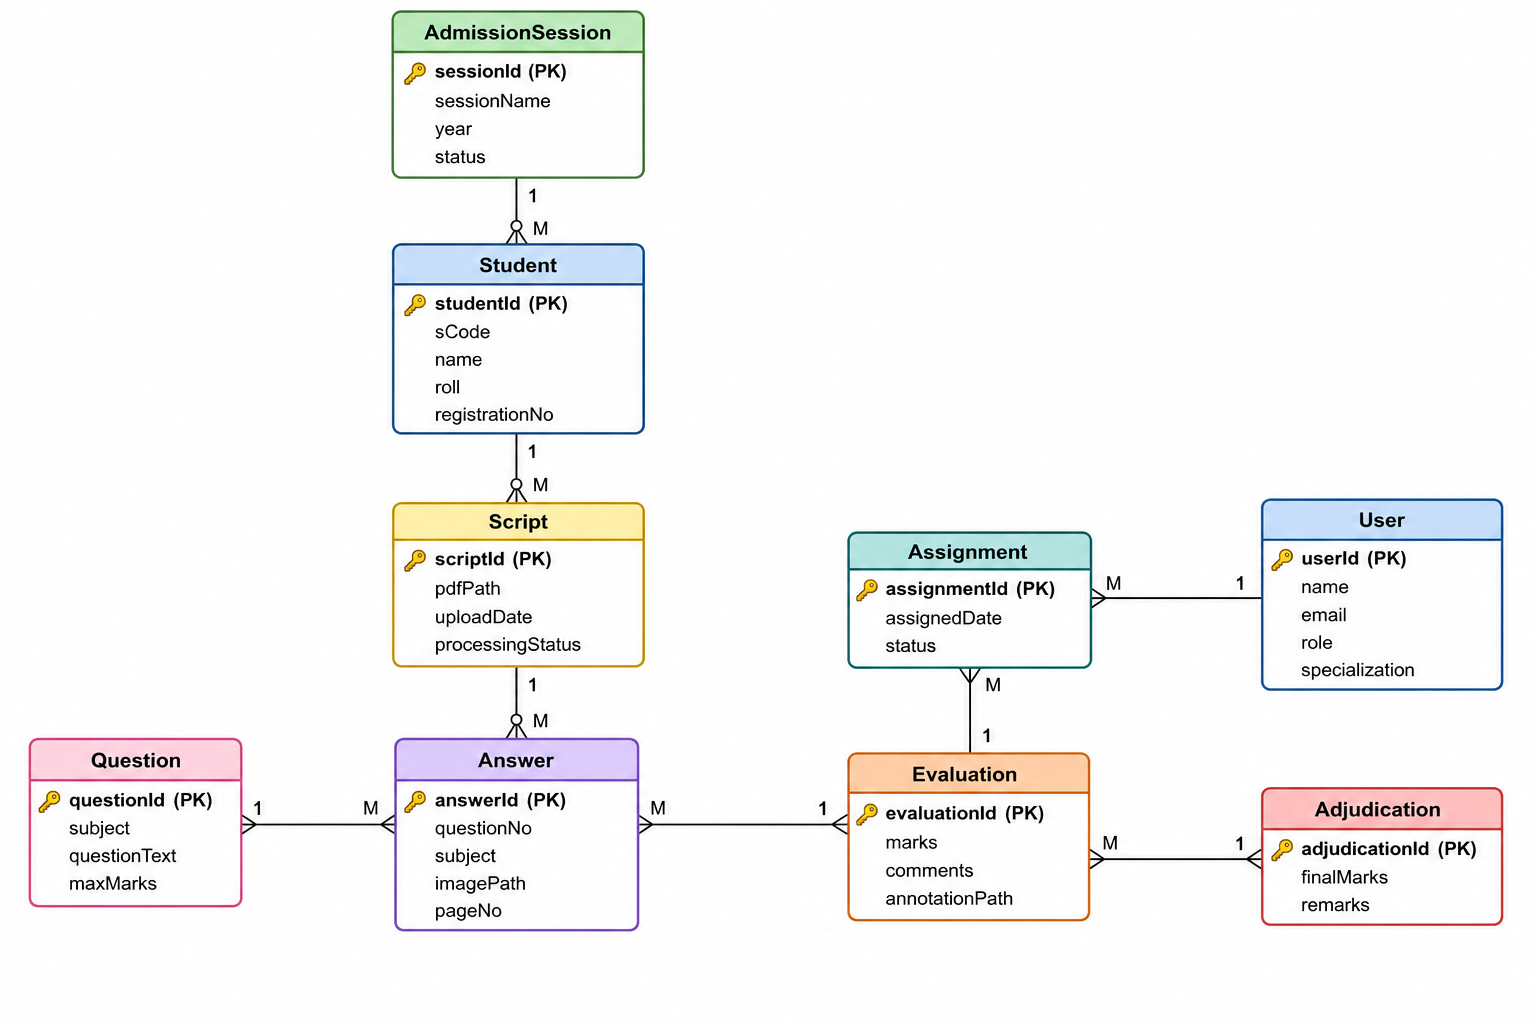
\includegraphics[width=0.90\textwidth]{img/ER_diagram.png}
    \caption{Conceptual database design of the proposed DASEMS.}
    \label{fig:database_design}
\end{figure}




\subsubsection{Database Collections}

The database consists of several major collections that support the admission evaluation workflow.

\begin{itemize}
    \item \textbf{User:} Stores authentication credentials, user profiles, and assigned roles.
    
    \item \textbf{Admission Session:} Maintains examination information including academic year, departments, schedule, and session status.
    
    \item \textbf{Question Bank:} Stores subject-wise questions, model answers, marking rubrics, and maximum marks.
    
    \item \textbf{Student:} Contains student information together with an anonymous identifier (\textbf{s\_code}) used during evaluation.
    
    \item \textbf{Script and Answer:} Store uploaded PDF information and extracted question-wise answer images with their metadata.
    
    \item \textbf{Assignment, Evaluation, and Moderation:} Manage teacher assignments, submitted marks, evaluation records, and moderation decisions.
    
    \item \textbf{Audit Log:} Records important system activities for transparency and future verification.
\end{itemize}

\subsubsection{Entity Relationships}

Each admission session contains multiple students, subjects, and questions. Every student is linked to one uploaded answer script, which is segmented into multiple question-wise answers. Each extracted answer is assigned to three teachers, producing independent evaluation records. When the submitted marks exceed the moderation threshold, the answer is forwarded to the Head Examiner for review. Finalized evaluations are then associated with the corresponding student for result generation, while all activities are recorded in the audit log.

% \subsubsection{Database Design Considerations}

% The database is designed with scalability, performance, and maintainability in mind. Frequently accessed collections are indexed to improve query performance, while uploaded PDFs and answer images are stored separately from the database, with only their metadata being maintained. Evaluation records are treated as immutable to preserve academic integrity, and append-only audit logs ensure complete traceability of all operations.

\subsection{OCR-Based PDF Processing Pipeline}

The OCR-Based PDF Processing Pipeline is the core document processing component of the proposed \textbf{Digital Admission Script Evaluation and Moderation System (DASEMS)}. Its objective is to convert uploaded admission answer scripts into question-wise answer images for digital evaluation. Instead of recognizing handwritten answers, the pipeline identifies question boundaries, extracts answer regions, and generates metadata while preserving the original uploaded PDF.

To improve efficiency, the system adopts a hybrid processing strategy. If the uploaded PDF contains an embedded searchable text layer, question locations are obtained directly using PDF processing libraries. Otherwise, the system automatically applies Optical Character Recognition (OCR) to detect printed question numbers from rendered page images. This approach enables reliable processing of both digital and scanned documents.

% Figure~\ref{fig:ocr_pipeline} illustrates the overall OCR-based processing pipeline.

% \begin{figure}[ht]
%     \centering
%     \includegraphics[width=0.90\textwidth]{img/ocr_pipeline.png}
%     \caption{OCR-Based PDF Processing Pipeline used in DASEMS.}
%     \label{fig:ocr_pipeline}
% \end{figure}

The pipeline consists of several sequential stages, beginning with PDF upload and ending with the generation of structured answer records.

\subsubsection{PDF Upload and Validation}

The pipeline begins when the Super Administrator uploads a PDF answer script. The system validates the file format, integrity, page structure, and admission session before storing the original PDF as a read-only document. This ensures data integrity and prevents invalid files from entering the processing pipeline.

\subsubsection{PDF Rendering}

Validated PDF pages are rendered into high-resolution images using the PyMuPDF library. These images provide the input for OCR and answer extraction when searchable text is unavailable.

\begin{figure}[H]
\centering

\begin{tikzpicture}[
    >=Stealth,
    node distance=0.9cm,
    box/.style={
        rectangle,
        rounded corners=6pt,
        minimum width=5cm,
        minimum height=0.9cm,
        draw=black,
        thick,
        align=center,
        font=\bfseries
    },
    smallbox/.style={
        rectangle,
        rounded corners=5pt,
        minimum width=3.2cm,
        minimum height=0.8cm,
        draw=black,
        thick,
        align=center,
        font=\small\bfseries
    },
    arrow/.style={
        ->,
        thick
    }
]

% Main Flow
\node[box,fill=blue!20] (upload) {PDF Upload};

\node[box,fill=green!20,below=of upload] (validation)
{File Validation};

\node[box,fill=yellow!25,below=of validation] (store)
{Store Original PDF};

\node[box,fill=orange!25,below=of store] (render)
{PDF Rendering};

% Text Layer Detection
\node[box,fill=cyan!25,below=of render] (textlayer)
{Text Layer Detection};

% Branches
\node[smallbox,fill=green!15] (text)
at (-3,-6)
{Question\\Detection};

\node[smallbox,fill=red!15] (ocr)
at (3,-6)
{OCR\\Detection};

% Merge
\node[box,fill=purple!20] (boundary)
at (0,-8)
{Question Boundary Identification};

\node[box,fill=orange!20,below=of boundary]
(crop){Answer Region Cropping};

\node[box,fill=pink!20,below=of crop]
(meta){Metadata Generation};

\node[box,fill=teal!20,below=of meta]
(records){Answer Records Created};

% Connections
\draw[arrow] (render)--(textlayer);

\draw[arrow] (textlayer)--node[left]{\scriptsize Text}(text);

\draw[arrow] (textlayer)--node[right]{\scriptsize No Text}(ocr);

\draw[arrow] (text)--(boundary);

\draw[arrow] (ocr)--(boundary);

\draw[arrow] (boundary)--(crop);

\draw[arrow] (crop)--(meta);

\draw[arrow] (meta)--(records);

\end{tikzpicture}

\caption{PDF Processing and Answer Extraction Workflow}
\label{fig:pdf_processing_workflow}

\end{figure}

\subsubsection{Question Detection}

Question detection is performed using a hybrid two-stage approach. The processor first attempts to extract embedded PDF text and its positional coordinates. If no searchable text exists, OCR is applied to the rendered page images to detect printed question numbers and their locations. This strategy improves both processing speed and robustness.

\subsubsection{Answer Region Extraction}

Using the detected question positions, the system determines the boundary of each answer region, crops it as an independent image, and generates metadata including the anonymous student identifier, subject, question number, page number, coordinates, and image location. These records are stored for teacher assignment and evaluation while the original PDF remains unchanged.

\subsubsection{Advantages of the Proposed Pipeline}

The proposed pipeline preserves the original answer script, automates question-wise answer extraction, and reduces administrative effort. The hybrid strategy avoids unnecessary OCR operations while supporting both searchable and scanned PDFs. The extracted answer images become independent evaluation units that enable automatic teacher assignment, parallel evaluation, and efficient moderation for large-scale admission examinations.

\subsubsection*{Algorithm 3.1: OCR-Based Answer Extraction}

\begin{verbatim}
Input:
    Uploaded PDF document

Output:
    Question-wise extracted answer images

Begin

Validate uploaded PDF

Store original PDF

For each page in the document do

    If searchable text exists then

        Extract text layer
        Detect question positions

    Else

        Render page image
        Perform OCR
        Detect question positions

    End If

    Identify answer boundaries

    Crop answer regions

    Save extracted answer image

    Generate metadata

End For

Store extracted answer records

Return extracted answers

End
\end{verbatim}



\subsection{Teacher Assignment and Moderation Algorithm}

After question-wise answer extraction, the proposed system automatically assigns each answer to qualified teachers for evaluation. The assignment mechanism ensures subject compatibility, balanced workload distribution, and independent evaluation while reducing the administrative effort associated with manual script distribution.

Each extracted answer contains metadata such as subject, question number, anonymous student identifier, and answer image location. Based on the subject, the system retrieves eligible teachers and assigns the answer to three evaluators with the lowest current workload. Teachers can access only their assigned answers and cannot view the evaluations submitted by others, ensuring unbiased assessment.

\subsubsection*{Algorithm 3.2: Teacher Assignment}

\begin{verbatim}
Input : Extracted Answer, Teacher List
Output: Three Assignment Records

Retrieve teachers by subject
Sort by current workload
Assign first three teachers
Store assignment records
Return assignments
\end{verbatim}

\subsubsection{Moderation Process}

To improve evaluation reliability, every answer is independently evaluated by three teachers. After all evaluations are submitted, the system calculates the mark spread:

\begin{equation}
Spread=\max(M_1,M_2,M_3)-\min(M_1,M_2,M_3)
\end{equation}

If

\begin{equation}
Spread \leq T
\end{equation}

the final mark is calculated as

\begin{equation}
FinalMark=\frac{M_1+M_2+M_3}{3}
\end{equation}

Otherwise, the answer is forwarded to the Head Examiner for moderation. The Head Examiner reviews the extracted answer, marking rubric, teacher annotations, comments, and assigned marks before determining the final score. The moderation decision is then stored in the database together with the review information.

\subsubsection*{Algorithm 3.3: Moderation Process}

\begin{verbatim}
Input : Three Teacher Evaluations
Output: Final Evaluation

Calculate mark spread

If spread <= threshold
    FinalMark = Average(M1,M2,M3)
Else
    Send to Head Examiner
    Receive moderated mark
End If

Store final result
\end{verbatim}

\subsection{Security and Authentication}

Security is a key aspect of the proposed \textbf{Digital Admission Script Evaluation and Moderation System (DASEMS)} as it handles confidential admission data and evaluation records.

The system uses encrypted password hashing for user authentication and JSON Web Tokens (JWT) for secure session management. Passwords are never stored in plain text, and only valid tokens are allowed to access protected resources.

Role-Based Access Control (RBAC) restricts system access according to user roles: \textbf{Super Administrator}, \textbf{Teacher}, and \textbf{Head Examiner}. Teachers can evaluate only assigned scripts, while student identities remain hidden through anonymous identifiers to ensure unbiased assessment.

\subsection{Deployment Architecture}

The proposed DASEMS adopts a modular deployment architecture that separates the frontend, backend, document processing service, and database into independent components. This design improves scalability, maintainability, and deployment flexibility.

% Figure~\ref{fig:deployment_architecture} illustrates the deployment architecture of the proposed system.


\begin{figure}[H]
\centering
\begin{tikzpicture}[
    >=Stealth,
    node distance=1.4cm,
    box/.style={
        draw,
        rounded corners,
        thick,
        minimum width=4cm,
        minimum height=1cm,
        align=center,
        font=\bfseries
    },
    smallbox/.style={
        draw,
        rounded corners,
        thick,
        minimum width=3cm,
        minimum height=0.8cm,
        align=center,
        font=\small
    },
    arrow/.style={->,thick}
]

% Main Components
\node[box,fill=blue!20] (frontend) {React Frontend};

\node[box,fill=green!20,below=of frontend] (backend)
{Node.js API Server};

\node[box,fill=orange!20,below left=1.6cm and 2.5cm of backend] (db)
{MongoDB};

\node[box,fill=purple!20,below right=1.6cm and 2.5cm of backend] (python)
{Python Processor};

% Subcomponents
\node[smallbox,fill=orange!10,below=0.9cm of db] (uploads)
{Uploads\\Images};

\node[smallbox,fill=purple!10,below=0.9cm of python] (ocr)
{OCR\\Cropping};

% Connections
\draw[arrow] (frontend) -- (backend);

\draw[arrow] (backend) -- (db);
\draw[arrow] (backend) -- (python);

\draw[arrow] (db) -- (uploads);
\draw[arrow] (python) -- (ocr);

\end{tikzpicture}
\caption{Overall System Component Architecture}
\label{fig:system_component_architecture}
\end{figure}


% \begin{figure}[ht]
%     \centering
%     \includegraphics[width=0.90\textwidth]{img/deployment_architecture.png}
%     \caption{Deployment architecture of the proposed DASEMS.}
%     \label{fig:deployment_architecture}
% \end{figure}



The frontend is developed using React and TypeScript, while the backend is implemented with Node.js and Express.js to manage authentication, evaluation, moderation, and system APIs.

A separate Python service performs PDF processing, OCR, question detection, and answer extraction independently of the web server. MongoDB stores user information, examination data, evaluations, moderation records, and final results. All major services are containerized using Docker to simplify deployment and improve portability. 




\mychapter{Implementation}
\vspace{0.5cm}

\subsection{Introduction}

This chapter presents the implementation of the proposed \textbf{Digital Admission Script Evaluation and Moderation System (DASEMS)}. The system was developed as a web-based platform to automate the workflow of descriptive admission script evaluation.

The implementation follows a modular architecture comprising a React frontend, Node.js and Express.js backend, MongoDB database, and a Python-based document processing service for PDF analysis and answer extraction. These components communicate through RESTful APIs to ensure efficient integration and scalability.

The system supports admission management, PDF processing, teacher assignment, evaluation, moderation, and result generation, while preserving human judgment during answer assessment. The following sections describe the development environment and implementation techniques used in the proposed system.


\subsection{Development Environment}

The proposed \textbf{Digital Admission Script Evaluation and Moderation System (DASEMS)} was developed using a modern full-stack technology stack suitable for web-based applications and document processing.

The frontend was implemented using \textbf{React 18} and \textbf{TypeScript}, while the backend was developed using \textbf{Node.js} and \textbf{Express.js}. \textbf{MongoDB} was selected as the primary database because of its flexible document-oriented architecture. A separate Python service built with \textbf{FastAPI} performs PDF processing, OCR, and image analysis using libraries such as \textbf{PyMuPDF}, \textbf{pdfplumber}, \textbf{Pillow}, and \textbf{Tesseract OCR}.

Docker Compose was used to containerize the backend, database, Redis cache, and Python processing service, ensuring consistent deployment across different environments. Git was used for version control, while Visual Studio Code served as the primary development environment.


\begin{table}[ht]
\centering
\caption{Summarizes the technologies used during system development.}
\label{tab:development_environment}

\begin{tabular}{|p{5cm}|p{7cm}|}
\hline
\textbf{Component} & \textbf{Technology Used} \\
\hline
Programming Language & TypeScript, JavaScript, Python \\
\hline
Frontend Framework & React 18 \\
\hline
Backend Framework & Node.js, Express.js \\
\hline
Database & MongoDB \\
\hline
Document Processor & Python FastAPI \\
\hline
OCR Engine & Tesseract OCR \\
\hline
PDF Processing & PyMuPDF, pdfplumber \\
\hline
Image Processing & Pillow \\
\hline
Authentication & JWT, bcrypt \\
\hline
State Management & Redux Toolkit \\
\hline
API Communication & React Query \\
\hline
Styling & Tailwind CSS \\
\hline
Annotation Library & React Konva \\
\hline
Containerization & Docker Compose \\
\hline
Version Control & Git \\
\hline
Development Environment & Visual Studio Code \\
\hline
\end{tabular}
\end{table}

The complete system was developed and tested on a macOS environment, with Docker Compose managing communication among all services to provide a consistent and reliable development platform.

\subsection{Backend Implementation}

The backend is the core component of the proposed \textbf{Digital Admission Script Evaluation and Moderation System (DASEMS)}. It manages communication among the frontend, MongoDB database, and Python document processing service while implementing the system's business logic.

Developed using \textbf{Node.js} and \textbf{Express.js}, the backend follows a modular architecture with controllers, services, repositories, models, and middleware. It supports authentication, student and admission management, answer script processing, teacher assignment, evaluation, moderation, and reporting.

The following subsections describe the backend structure, authentication mechanism, and REST API implementation.


% flow chart
%===========================
% Preamble
%===========================

\usetikzlibrary{positioning,arrows.meta,calc}

%===========================
% Figure
%===========================
\begin{figure}[ht]
\centering
\resizebox{\textwidth}{!}{%
\begin{tikzpicture}[
    >=Stealth,
    node distance=1cm,
    box/.style={
        draw,
        rounded corners,
        thick,
        minimum width=2.8cm,
        minimum height=0.8cm,
        align=center,
        font=\small\bfseries
    },
    smallbox/.style={
        draw,
        rounded corners,
        thick,
        minimum width=2cm,
        minimum height=0.7cm,
        align=center,
        font=\scriptsize
    },
    arrow/.style={->,thick}
]

%------------------------------------------------
% Top Layer
%------------------------------------------------

\node[box,fill=blue!20] (app) {Express Application};

\node[box,fill=green!20,below=1.5cm of app] (config) {Configuration};

\node[box,fill=orange!20,left=5cm of config] (server)
{app.ts\\server.ts};

\node[box,fill=red!20,right=5cm of config] (middleware)
{Middleware};

\draw[arrow] (app) -- (config);
\draw[arrow] (app) -| (server);
\draw[arrow] (app) -| (middleware);

%------------------------------------------------
% Middleware
%------------------------------------------------

\node[smallbox,fill=red!10,below=0.7cm of middleware] (jwt)
{JWT Authentication};

\node[smallbox,fill=red!10,below=0.25cm of jwt] (role)
{Role Authorization};

\node[smallbox,fill=red!10,below=0.25cm of role] (req)
{Request Validation};

\node[smallbox,fill=red!10,below=0.25cm of req] (err)
{Error Handling};

\node[smallbox,fill=red!10,below=0.25cm of err] (audit)
{Audit Logging};

\draw[arrow] (middleware)--(jwt);
\draw[arrow] (jwt)--(role);
\draw[arrow] (role)--(req);
\draw[arrow] (req)--(err);
\draw[arrow] (err)--(audit);

%------------------------------------------------
% Router
%------------------------------------------------

\node[box,fill=cyan!20,below=3.2cm of config] (router)
{API Routing Layer};

\draw[arrow] (config)--(router);

%------------------------------------------------
% Modules
%------------------------------------------------

\node[smallbox,fill=yellow!20,below left=1.4cm and 6cm of router] (auth){Auth};
\node[smallbox,fill=yellow!20,right=0.8cm of auth] (users){Users};
\node[smallbox,fill=yellow!20,right=0.8cm of users] (students){Students};
\node[smallbox,fill=yellow!20,right=0.8cm of students] (questions){Questions};
\node[smallbox,fill=yellow!20,right=0.8cm of questions] (evaluation){Evaluation};
\node[smallbox,fill=yellow!20,right=0.8cm of evaluation] (results){Results};

\foreach \x in {auth,users,students,questions,evaluation,results}
\draw[arrow] (router.south)--(\x.north);

%------------------------------------------------
% Controllers
%------------------------------------------------

\foreach \x/\name in {
auth/authc,
users/usersc,
students/studentsc,
questions/questionsc,
evaluation/evaluationc,
results/resultsc}
{
\node[smallbox,fill=green!15,below=0.8cm of \x] (\name)
{Controllers};

\draw[arrow] (\x)--(\name);
}

%------------------------------------------------
% Services
%------------------------------------------------

\foreach \x/\name in {
authc/auths,
usersc/userss,
studentsc/studentss,
questionsc/questionss,
evaluationc/evaluations,
resultsc/resultss}
{
\node[smallbox,fill=orange!20,below=0.8cm of \x] (\name)
{Services};

\draw[arrow] (\x)--(\name);
}

%------------------------------------------------
% Repositories
%------------------------------------------------

\foreach \x/\name in {
auths/authr,
userss/usersr,
studentss/studentsr,
questionss/questionsr,
evaluations/evaluationr,
resultss/resultsr}
{
\node[smallbox,fill=purple!20,below=0.8cm of \x] (\name)
{Repositories};

\draw[arrow] (\x)--(\name);
}

%------------------------------------------------
% Database
%------------------------------------------------

\node[box,fill=teal!20,below=1.5cm of studentsr]
(mongoose){Mongoose Models};

\node[box,fill=blue!15,below=1cm of mongoose]
(mongo){MongoDB Database};

\foreach \x in {authr,usersr,studentsr,questionsr,evaluationr,resultsr}
{
\draw[arrow] (\x.south)|-(mongoose.north);
}

\draw[arrow] (mongoose)--(mongo);

\end{tikzpicture}
}
\caption{Express Backend Architecture}
\label{fig:express_backend}
\end{figure}

\subsubsection{Project Structure}

The backend follows a feature-oriented directory structure, where related files are grouped into independent modules for easier maintenance and future expansion.

The main directories are:

\begin{itemize}
\item \textbf{Config}: Configuration and database settings.
\item \textbf{Routes}: REST API endpoints.
\item \textbf{Controllers}: Request handling.
\item \textbf{Services}: Business logic.
\item \textbf{Repositories}: Database operations.
\item \textbf{Models}: MongoDB schemas.
\item \textbf{Middleware}: Authentication, authorization, and validation.
\end{itemize}

\subsubsection{Authentication and Authorization Module}

Authentication uses \textbf{JWT} with \textbf{bcrypt}-hashed passwords. After login, a JWT is issued and verified for every protected request. Authorization is enforced through \textbf{Role-Based Access Control (RBAC)}, supporting Super Administrator, Teacher, and Head Examiner roles with predefined permissions.

\subsubsection{REST API Implementation}

The frontend communicates with the backend through RESTful APIs using standard HTTP methods. Protected endpoints require JWT authentication and RBAC authorization. The APIs are organized into modules such as Authentication, User Management, Admission Session, Question Management, Student Management, Document Processing, Evaluation, Moderation, Reporting, and Audit Logging.

\begin{table}[H]
\centering
\caption{Major Backend Modules}
\label{tab:backend_modules}

\begin{tabular}{|p{5cm}|p{8cm}|}
\hline
\textbf{Module} & \textbf{Primary Responsibility} \\
\hline
Authentication & User login, JWT generation, token validation \\
\hline
User Management & Teacher and Head Examiner management \\
\hline
Admission Session & Admission session and examination configuration \\
\hline
Question Management & Question bank and marking rubric management \\
\hline
Student Management & Candidate registration and answer script upload \\
\hline
Document Processing & Coordination with the Python OCR processing service \\
\hline
Assignment & Automatic teacher allocation and workload distribution \\
\hline
Evaluation & Digital marking and evaluation submission \\
\hline
Moderation & Head Examiner review and final mark determination \\
\hline
Reporting & Result generation and analytical reports \\
\hline
Audit Logging & Recording system activities and user actions \\
\hline
\end{tabular}

\end{table}

\subsection{Frontend Implementation}

The frontend of the proposed \textbf{Digital Admission Script Evaluation and Moderation System (DASEMS)} was implemented as a Single Page Application (SPA) using \textbf{React 18} and \textbf{TypeScript}. It provides dedicated interfaces for Super Administrators, Teachers, and Head Examiners while communicating with backend services through RESTful APIs.

React's component-based architecture improves code reusability and application responsiveness by updating only the modified components. React Query manages asynchronous API communication and caching, while Redux Toolkit maintains authentication and global application state. Tailwind CSS is used for responsive interface design, and React Konva provides digital annotation tools for answer evaluation.


\begin{figure}[H]
\centering

\begin{tikzpicture}[
node distance=1.2cm,
box/.style={
    rectangle,
    rounded corners=6pt,
    minimum width=4.2cm,
    minimum height=1cm,
    draw=black,
    thick,
    font=\bfseries,
    align=center,
    drop shadow
},
smallbox/.style={
    rectangle,
    rounded corners=5pt,
    minimum width=3.2cm,
    minimum height=0.9cm,
    draw=black,
    thick,
    font=\bfseries,
    align=center,
    drop shadow
},
line/.style={
    -{Stealth[length=3mm]},
    thick
}
]

% Main Flow
\node[box,fill=blue!20] (react) {React Application};

\node[box,fill=green!20,below=of react] (router) {React Router};

% Dashboards
\node[smallbox,fill=orange!20,below left=1.6cm and 2.6cm of router] (admin)
{Admin\\Dashboard};

\node[smallbox,fill=yellow!25,below=1.8cm of router] (teacher)
{Teacher\\Dashboard};

\node[smallbox,fill=red!20,below right=1.6cm and 2.6cm of router] (head)
{Head Examiner\\Dashboard};

% Bottom
\node[box,fill=cyan!20,below=3cm of teacher] (api)
{REST API Services};

\node[box,fill=purple!20,below=of api] (backend)
{Express Backend};

% Connections
\draw[line] (react) -- (router);

\draw[line] (router) |- (admin);
\draw[line] (router) -- (teacher);
\draw[line] (router) |- (head);

\draw[line] (admin) |- (api);
\draw[line] (teacher) -- (api);
\draw[line] (head) |- (api);

\draw[line] (api) -- (backend);

\end{tikzpicture}

\caption{Frontend Architecture and Routing Workflow}
\label{fig:frontend_architecture}

\end{figure}


The frontend provides a consistent and responsive interface for managing the complete admission evaluation workflow.

\subsubsection{User Interface Design}

The interface follows a dashboard-based design in which users access only the functions permitted by their assigned roles. After authentication, users are automatically redirected to their respective dashboards. Navigation is kept simple through responsive layouts, tables, cards, and dialogs, ensuring efficient operation across desktop computers, laptops, and graphics tablets.

\subsubsection{Administrative Dashboard}

The Administrative Dashboard enables Super Administrators to manage admission sessions, users, departments, subjects, question banks, student registration, answer script uploads, evaluation progress, and result generation.

Real-time statistics, notifications, and progress indicators help administrators monitor processing status, pending evaluations, moderation requests, and overall examination activities from a centralized interface.

\subsubsection{Teacher Evaluation Workspace}

Teachers access only their assigned answers through a personalized evaluation workspace. Each evaluation page displays the question, model answer, marking rubric, anonymous student identifier, extracted answer image, annotation tools, mark entry field, and comment section.

Using React Konva, teachers can annotate answer images without modifying the original document. After submitting marks, the system automatically loads the next assigned answer, enabling efficient continuous evaluation.

\subsubsection{Head Examiner Dashboard}

The Head Examiner Dashboard manages answers requiring moderation. It displays the extracted answer image, model answer, marking rubric, marks from all evaluators, comments, and annotation layers. After reviewing the submitted evaluations, the Head Examiner assigns the final moderated mark, which is stored together with moderation remarks and timestamps.

\subsubsection{Frontend Communication}

The frontend communicates with backend services through RESTful APIs secured by JWT authentication. React Query handles asynchronous requests, caching, and automatic data synchronization, while Redux Toolkit manages user sessions and authentication state. Together, these technologies provide a responsive, secure, and maintainable frontend suitable for large-scale admission examinations.


\subsection{Database Implementation}

The proposed \textbf{Digital Admission Script Evaluation and Moderation System (DASEMS)} uses \textbf{MongoDB} as its primary database because of its flexible document-oriented architecture. MongoDB efficiently manages heterogeneous educational data, including users, admission sessions, question banks, students, answer scripts, evaluations, moderation records, and audit logs. Database operations are implemented using \textbf{Mongoose}, which provides schema validation, object modeling, and simplified interaction with MongoDB collections.

\subsubsection{Collection Implementation}

Each major system entity is implemented as a separate MongoDB collection to improve maintainability and scalability. The principal collections include:

\begin{itemize}
    \item \textbf{Users}: Authentication credentials, user profiles, and roles.
    \item \textbf{Admission Sessions}: Examination configuration and session information.
    \item \textbf{Questions}: Question bank, model answers, and marking rubrics.
    \item \textbf{Students}: Student information with anonymous identifiers (\textbf{s\_code}).
    \item \textbf{Scripts} and \textbf{Answers}: Uploaded PDFs and extracted question-wise answer images.
    \item \textbf{Assignments}, \textbf{Evaluations}, and \textbf{Adjudications}: Teacher assignments, submitted marks, and moderation records.
    \item \textbf{Audit Logs}: System activities and administrative actions.
\end{itemize}

\subsubsection{Relationship Implementation}

Logical relationships among collections are maintained using MongoDB document references. Each student belongs to an admission session and is associated with one uploaded script. Every script is segmented into multiple answers, which are assigned to three teachers for independent evaluation. When the moderation threshold is exceeded, evaluation records are linked to an adjudication record maintained by the Head Examiner.

Figure~\ref{fig:mongodb_relationships} illustrates the relationships among the primary MongoDB collections.

\begin{figure}[ht]
    \centering
    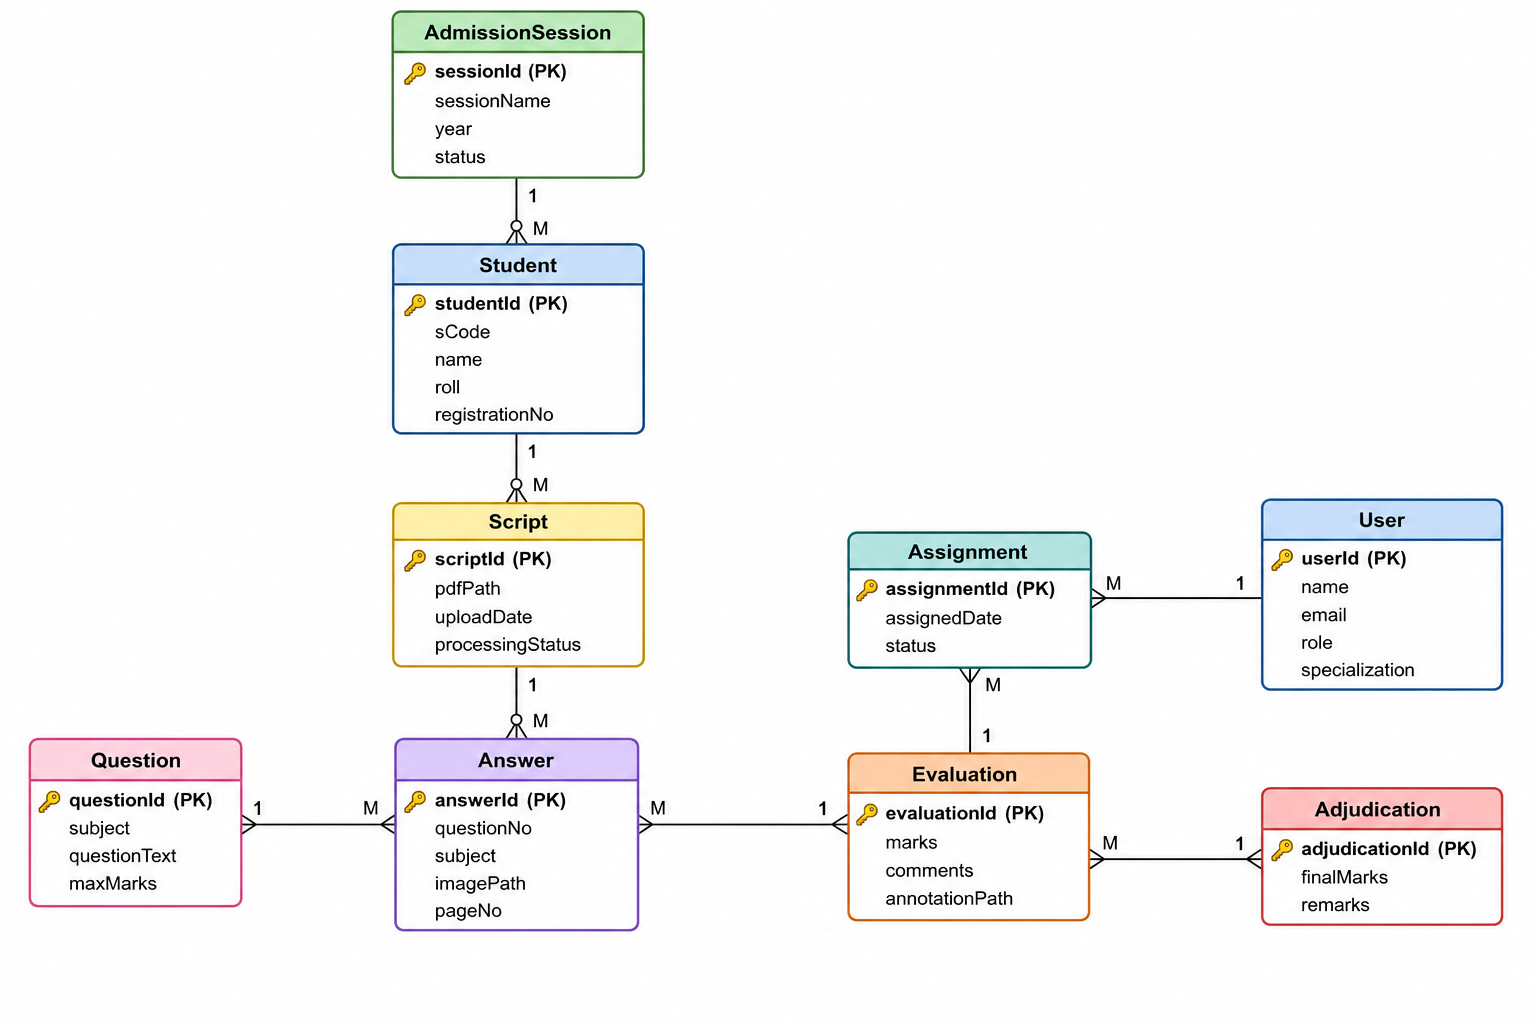
\includegraphics[width=0.90\textwidth]{img/ER_diagram.png}
    \caption{Logical relationships among the primary MongoDB collections.}
    \label{fig:mongodb_relationships}
\end{figure}


\subsubsection{Data Integrity and Consistency}

Mongoose schema validation ensures that all documents satisfy predefined constraints before insertion. Evaluation records remain immutable after submission, while moderation decisions are stored separately to preserve evaluation history. Audit logs follow an append-only strategy, ensuring complete traceability of system activities. Anonymous student identifiers further protect privacy by preventing teachers from accessing personal information during evaluation.

\subsection{PDF Processing Module}

The PDF Processing Module is the core component of the proposed \textbf{Digital Admission Script Evaluation and Moderation System (DASEMS)}. It converts uploaded admission answer scripts into question-wise answer records for digital evaluation. Implemented as an independent Python service, the module performs document validation, page rendering, hybrid question detection, answer extraction, metadata generation, and database integration. By separating document processing from the backend, computationally intensive OCR tasks do not affect application responsiveness.

Unlike conventional OCR-only approaches, the proposed module adopts a hybrid strategy. Searchable PDF text is extracted directly whenever available, while OCR is used only for scanned documents without an embedded text layer. This improves both processing speed and detection accuracy.



% \begin{figure}[ht]
%     \centering
%     \includegraphics[width=0.90\textwidth]{img/pdf_processing_workflow.png}
%     \caption{Implementation workflow of the PDF processing module.}
%     \label{fig:pdf_processing_workflow}
% \end{figure}

\begin{figure}[ht]
\centering

\begin{tikzpicture}[
    node distance=8mm,
    box/.style={
        rectangle,
        rounded corners=6pt,
        minimum width=8cm,
        minimum height=1cm,
        align=center,
        draw=black,
        thick,
        font=\bfseries,
        drop shadow
    },
    line/.style={
        -{Stealth[length=3mm]},
        thick
    }
]

\node[box,fill=blue!15] (A) {PDF Upload};
\node[box,fill=green!15,below=of A] (B) {File Validation};
\node[box,fill=yellow!25,below=of B] (C) {Store Original PDF};
\node[box,fill=orange!25,below=of C] (D) {Render PDF Pages};
\node[box,fill=red!15,below=of D] (E) {Question Detection};
\node[box,fill=purple!15,below=of E] (F) {Answer Region Identification};
\node[box,fill=cyan!20,below=of F] (G) {Answer Image Cropping};
\node[box,fill=pink!20,below=of G] (H) {Metadata Generation};
\node[box,fill=teal!20,below=of H] (I) {Database Storage};

\draw[line] (A) -- (B);
\draw[line] (B) -- (C);
\draw[line] (C) -- (D);
\draw[line] (D) -- (E);
\draw[line] (E) -- (F);
\draw[line] (F) -- (G);
\draw[line] (G) -- (H);
\draw[line] (H) -- (I);

\end{tikzpicture}

\caption{PDF Processing Workflow}
\label{fig:pdf_workflow}

\end{figure}



\subsubsection{PDF Upload and Validation}

The uploaded PDF is validated for file integrity, format, and readability before processing. Each document is linked to the corresponding admission session and anonymous student identifier (\textbf{s\_code}), while the original PDF is stored without modification to preserve authenticity throughout the evaluation process.

\subsubsection{PDF Rendering}

Each PDF page is converted into a high-resolution image using PyMuPDF. These rendered images provide a standardized input for OCR and subsequent image-processing operations while preserving the original document layout.

\subsubsection{Hybrid Question Detection}

The processor first attempts to extract embedded text directly from the PDF. If searchable text is unavailable, OCR is applied to detect printed question numbers and their coordinates. This hybrid approach ensures reliable processing for both digitally generated and scanned answer scripts while minimizing unnecessary OCR operations.



\begin{figure}[H]
    \centering
    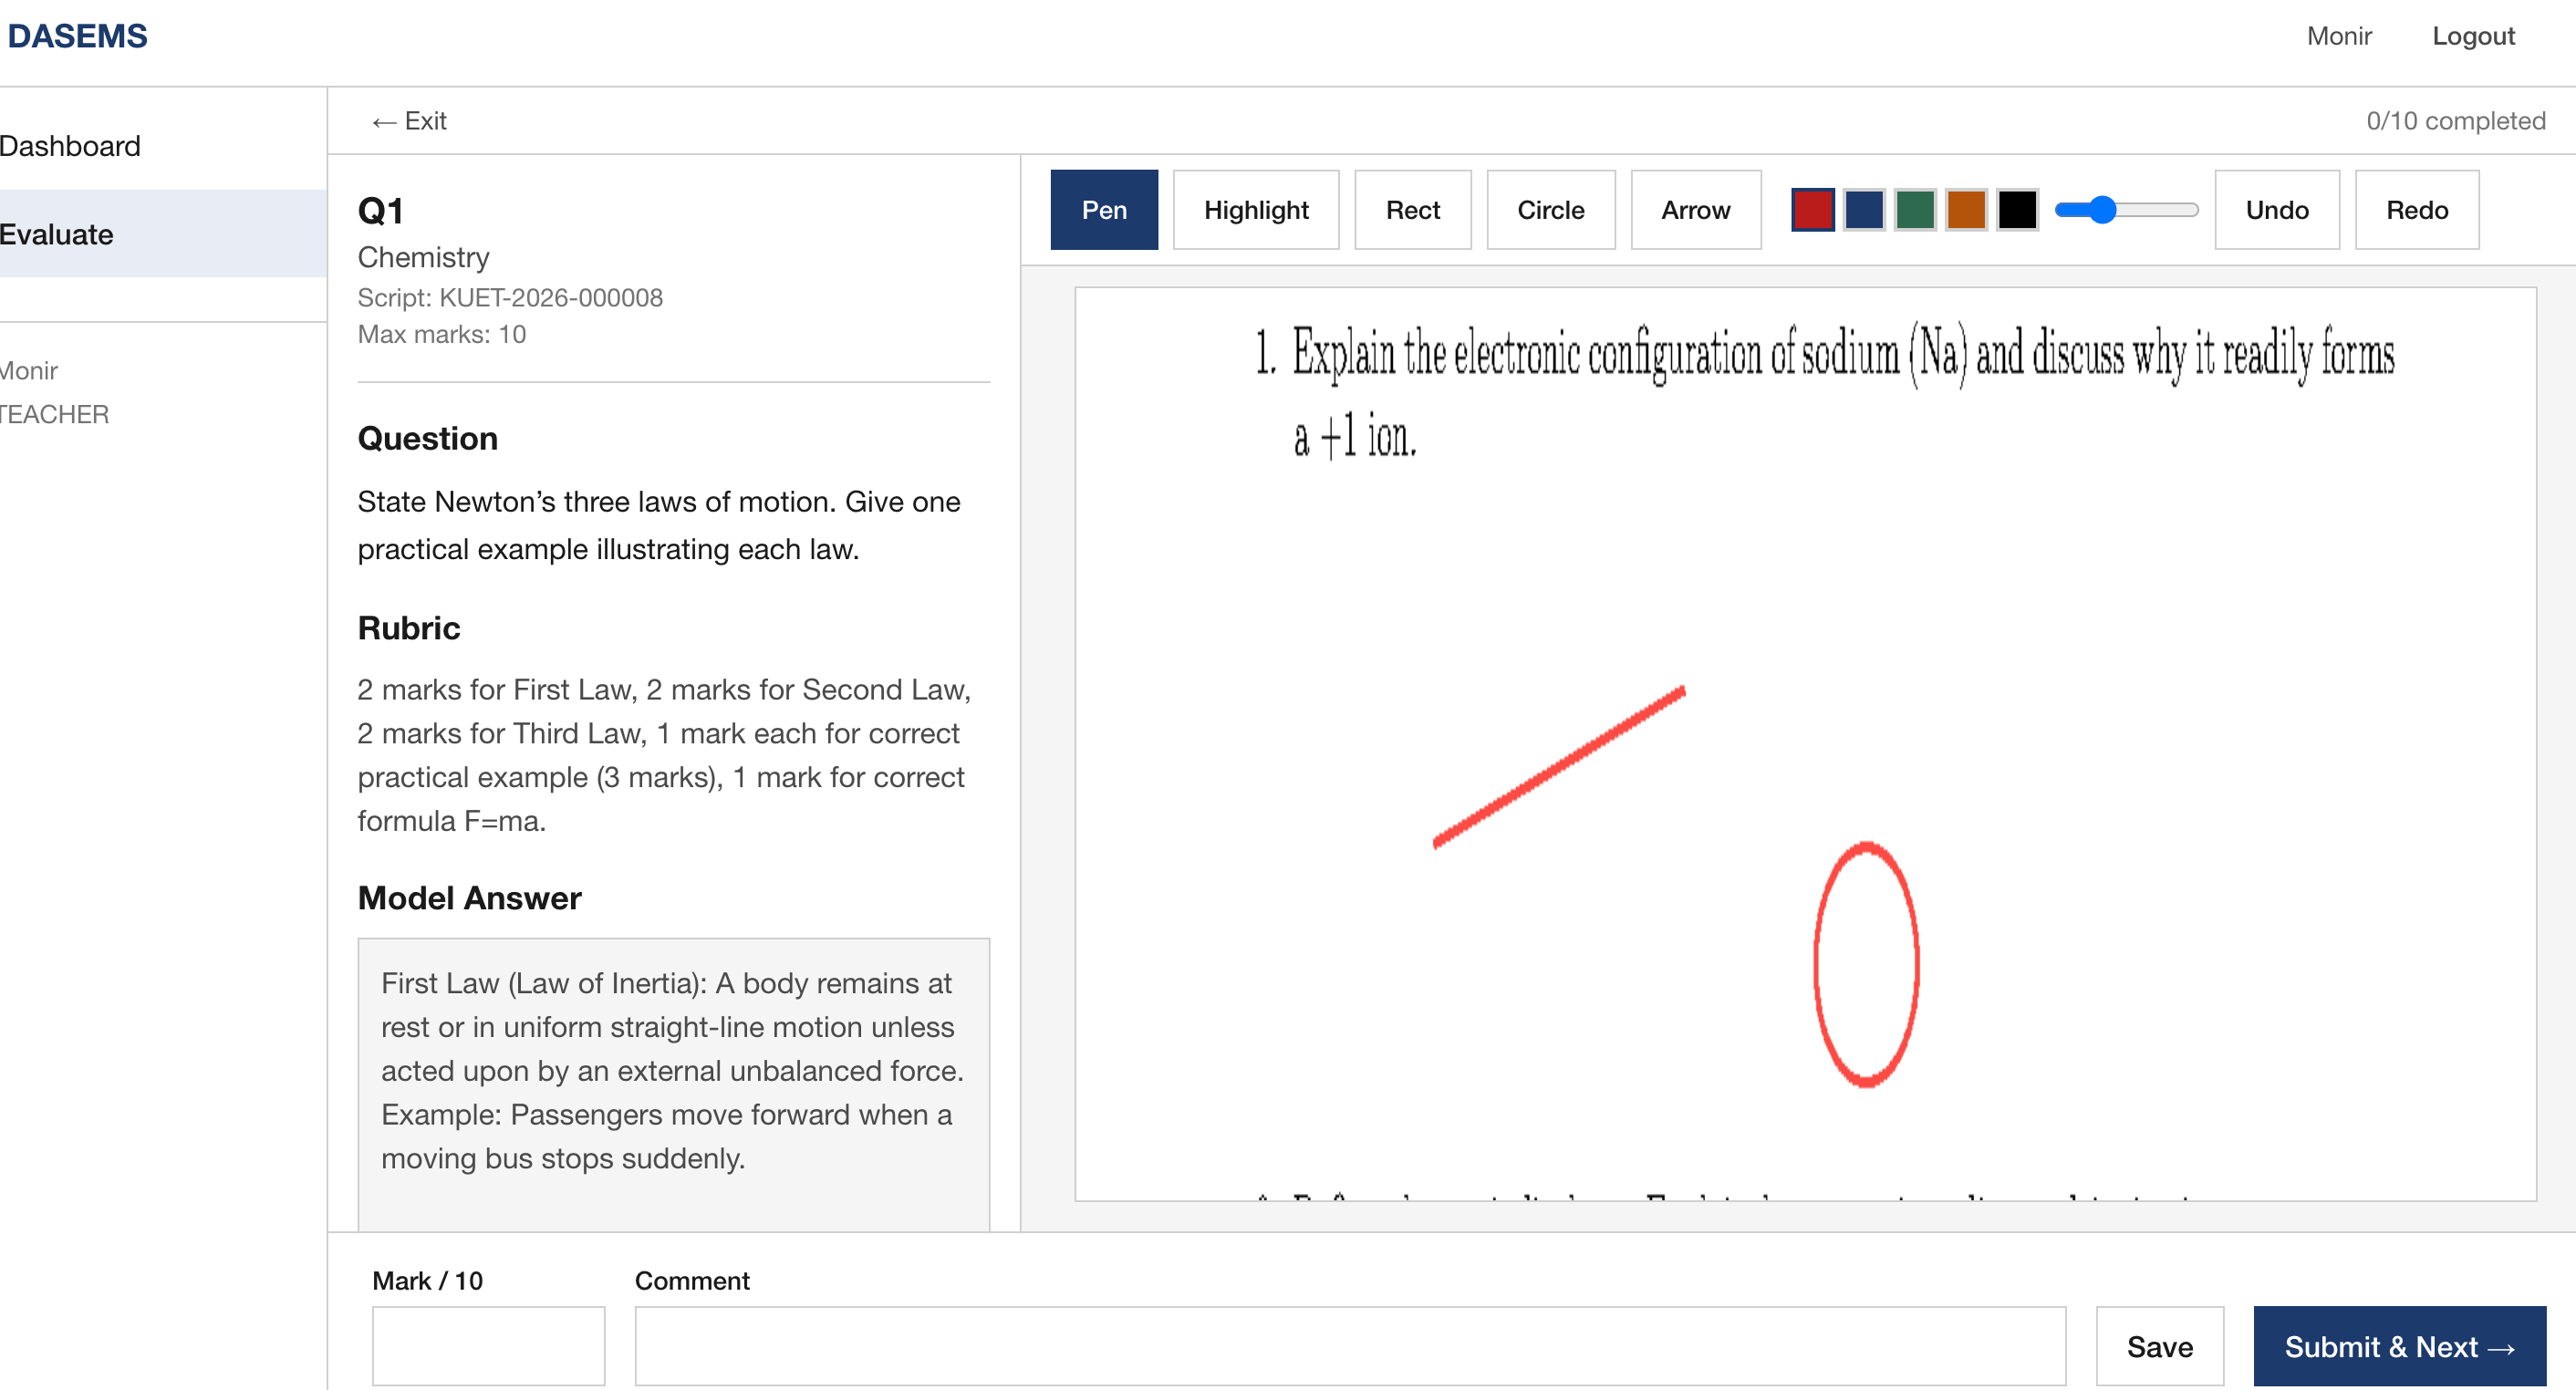
\includegraphics[width=0.90\textwidth]{img/question_detection.png}
    \caption{Hybrid question detection using PDF text extraction and OCR.}
    \label{fig:question_detection}
\end{figure}

\subsubsection{Answer Region Identification}

Using the detected question positions, the processor dynamically determines answer boundaries. Each answer begins below its corresponding question and extends to the next detected question or the end of the page. Multi-page answers are handled automatically, allowing answers of varying lengths to be extracted correctly.



\begin{figure}[H]
    \centering
    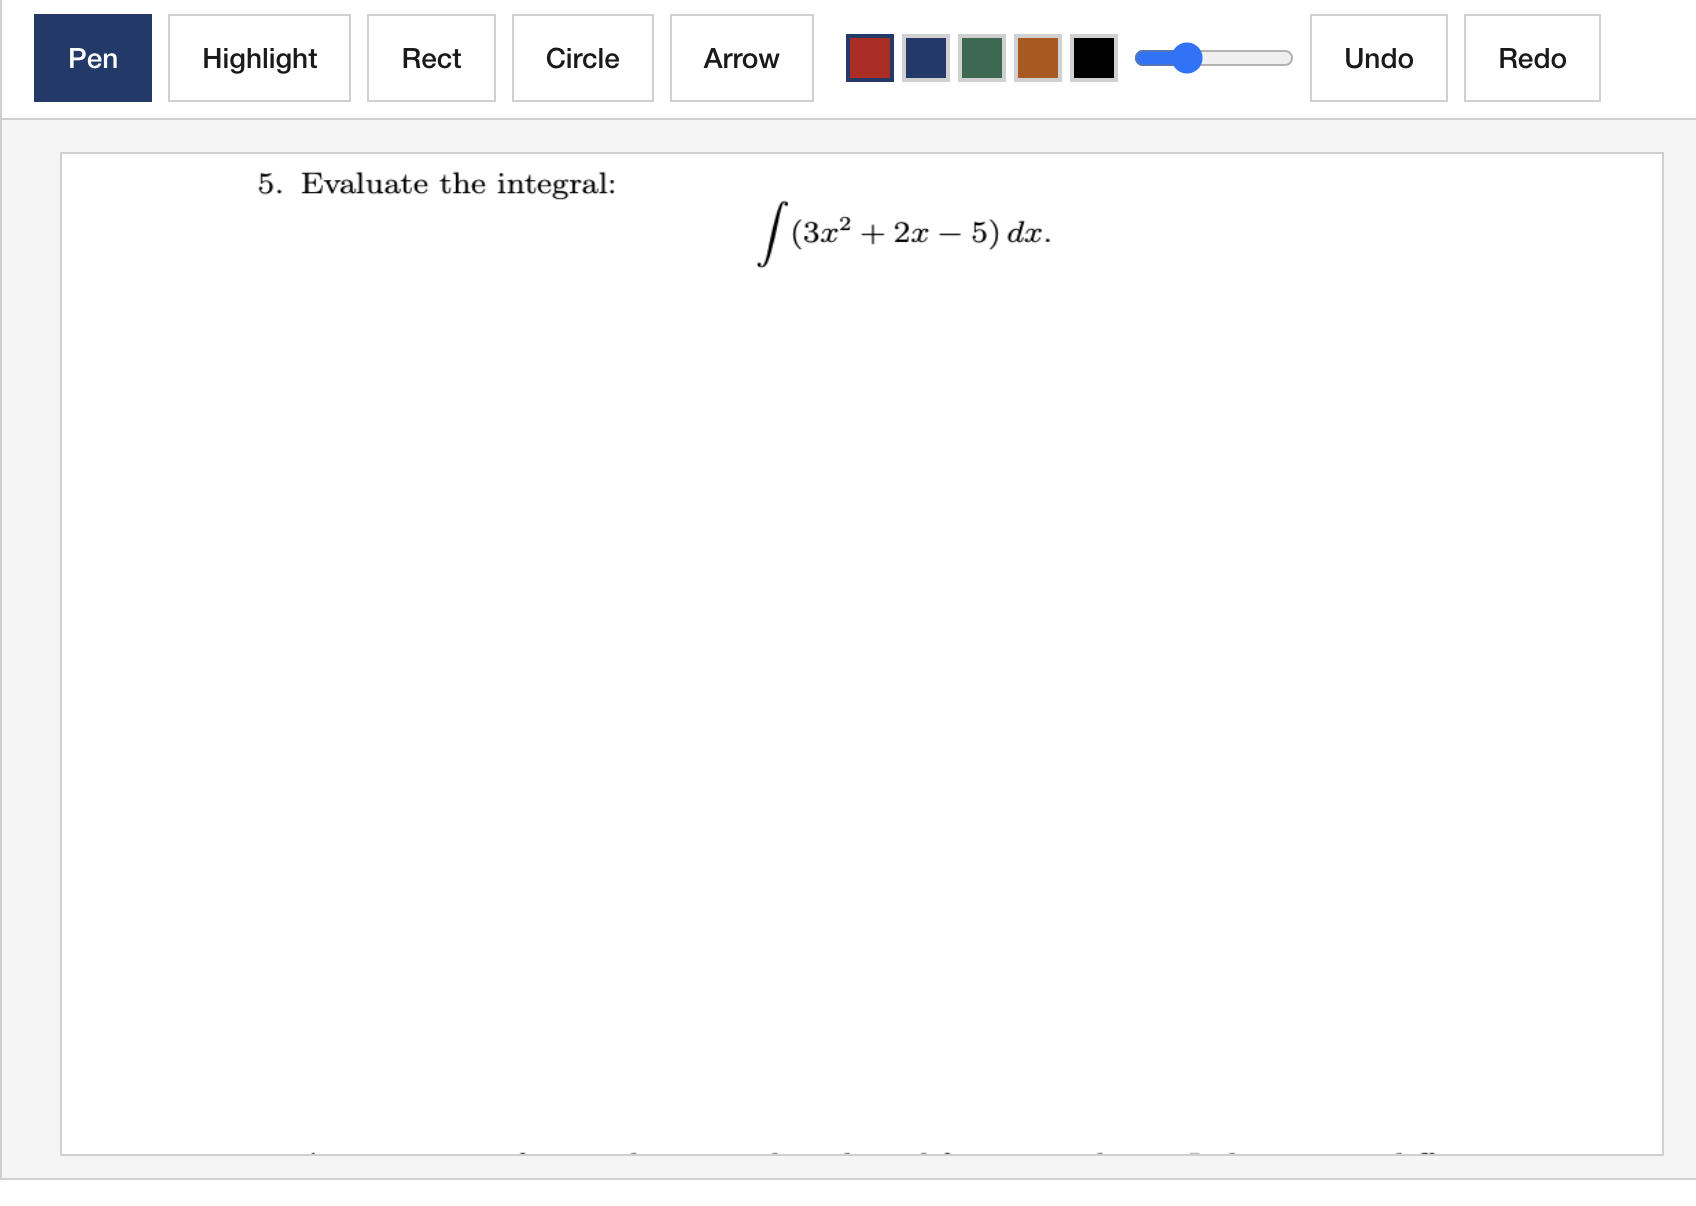
\includegraphics[width=0.85\textwidth]{img/question_detection1.png}
    \caption{Dynamic identification of answer boundaries based on detected question positions.}
    \label{fig:answer_segmentation}
\end{figure}

\subsubsection{Answer Extraction and Metadata Generation}

The identified answer regions are cropped using the Pillow library and stored as independent images. For each extracted answer, the processor generates metadata including the anonymous student identifier, subject, question number, page number, bounding coordinates, image location, and processing status. The metadata are transmitted to the backend as JSON objects for database storage and automatic teacher assignment.

\subsubsection{Database Integration}

The backend creates an independent database record for every extracted answer. Each record stores the extracted image reference, metadata, and processing status. These records serve as the primary evaluation units and are subsequently used for teacher assignment, evaluation, moderation, and result generation.

\subsubsection*{Algorithm 4.1: PDF Processing Pipeline}

\begin{verbatim}
Input:
    Uploaded PDF Document

Output:
    Question-wise Answer Records

Begin

Receive uploaded PDF
Validate document
Store original PDF
Render pages

For each page do

    Extract PDF text

    If unavailable
        Perform OCR
    End If

    Detect questions
    Determine answer boundaries
    Crop answers
    Generate metadata

End For

Store answer records
Return processing status

End
\end{verbatim}


\subsection{Teacher Assignment and Evaluation Implementation}

The proposed \textbf{Digital Admission Script Evaluation and Moderation System (DASEMS)} implements an automated teacher assignment mechanism to ensure fair, anonymous, and balanced evaluation of descriptive answers. After the PDF processing module extracts question-wise answers, the backend retrieves the associated metadata, including subject, question number, anonymous student identifier (\textbf{s\_code}), and answer image location. Based on the subject, the system automatically assigns answers to qualified teachers without manual intervention.

The assignment engine selects teachers according to their subject specialization and current evaluation workload to ensure balanced distribution. 

To maintain fairness, teachers evaluate answers using only the anonymous student identifier. The evaluation interface provides the extracted answer image, question statement, model answer, marking rubric, annotation tools, and mark submission form. Once submitted, evaluation records become read-only unless modified through the moderation process.

% for figure: 
\begin{figure}[H]
\centering

\begin{tikzpicture}[
    node distance=0.9cm,
    >=Stealth,
    process/.style={
        rectangle,
        rounded corners=8pt,
        draw=black!70,
        very thick,
        minimum width=8cm,
        minimum height=1cm,
        align=center,
        font=\bfseries,
        drop shadow
    },
    arrow/.style={
        ->,
        very thick,
        >=Stealth
    }
]

\node[process,fill=box1] (A) {Extracted Answer};

\node[process,fill=box2,below=of A] (B)
{Identify Subject};

\node[process,fill=box3,below=of B] (C)
{Retrieve Eligible Teachers};

\node[process,fill=box4,below=of C] (D)
{Check Current Workload};

\node[process,fill=box5,below=of D] (E)
{Assign to Three Teachers};

\node[process,fill=box6,below=of E] (F)
{Create Assignment Records};

\node[process,fill=box7,below=of F] (G)
{Teacher Evaluation Queue};

\draw[arrow] (A) -- (B);
\draw[arrow] (B) -- (C);
\draw[arrow] (C) -- (D);
\draw[arrow] (D) -- (E);
\draw[arrow] (E) -- (F);
\draw[arrow] (F) -- (G);

\end{tikzpicture}

\caption{Teacher Assignment Workflow}
\label{fig:teacher_assignment_workflow}

\end{figure}
\FloatBarrier




\subsubsection{Moderation Implementation}

To improve evaluation consistency, the system automatically compares the marks submitted by the three evaluators. If the difference between the highest and lowest marks is within the predefined moderation threshold, the final score is calculated as the average of the submitted marks.

When the variation exceeds the threshold, the answer is forwarded to the Head Examiner for moderation. The moderation dashboard displays the extracted answer image, model answer, marking rubric, teacher marks, comments, and annotations. After reviewing these materials, the Head Examiner assigns the final mark, which is permanently stored together with moderation remarks and timestamps.

The automated assignment and moderation mechanisms reduce administrative effort while improving fairness, transparency, and consistency throughout the admission evaluation process.



\subsection{Result Generation}

After teacher evaluation and moderation are completed, the proposed \textbf{Digital Admission Script Evaluation and Moderation System (DASEMS)} automatically generates the final admission examination results. The result generation module consolidates finalized evaluations, calculates student scores, and prepares administrative reports, thereby reducing manual effort and calculation errors.

Before generating results, the system verifies that all assigned evaluations and moderation tasks have been completed. If any answer remains pending, the corresponding student's result is withheld until the evaluation process is finalized. Once all evaluations are complete, the backend retrieves the approved marks for each question and automatically calculates the total score according to the examination rules.

% Figure~\ref{fig:result_generation} illustrates the workflow of the result generation module.

% \begin{figure}[ht]
%     \centering
%     \includegraphics[width=0.85\textwidth]{img/result_generation_workflow.png}
%     \caption{Workflow of the result generation module.}
%     \label{fig:result_generation}
% \end{figure}




The generated results are stored in the MongoDB database and displayed through the administrative dashboard. Administrators can access merit lists, subject-wise performance summaries, and complete evaluation histories for verification.

The reporting module also provides statistics such as:

\begin{itemize}
    \item Total evaluated answer scripts.
    \item Pending evaluations.
    \item Moderated answers.
    \item Subject-wise performance.
    \item Teacher workload.
    \item Final examination results.
\end{itemize}

By combining automatic score calculation with centralized reporting, the implemented module improves the efficiency, accuracy, and transparency of the admission evaluation process.


\subsection{System Testing and Validation}

After implementing all software modules, comprehensive testing was conducted to verify the correctness, reliability, and integration of the proposed \textbf{Digital Admission Script Evaluation and Moderation System (DASEMS)}. The testing process ensured that each module satisfied the functional requirements identified during system analysis.

Initially, unit testing was performed on individual modules, including authentication, admission management, PDF processing, answer extraction, teacher assignment, evaluation, moderation, and result generation. Integration testing was then conducted to verify communication among the React frontend, Node.js backend, Python document processing service, and MongoDB database.

Table~\ref{tab:functional_testing} summarizes the functional testing results.

\begin{table}[ht]
\centering
\caption{Functional Testing Results}
\label{tab:functional_testing}

\begin{tabular}{|p{6cm}|p{6cm}|p{2cm}|}
\hline
\textbf{System Function} & \textbf{Expected Outcome} & \textbf{Result} \\
\hline
User Login & Authorized user access & Pass \\
\hline
JWT Authentication & Secure API access & Pass \\
\hline
Admission Session Creation & Session stored successfully & Pass \\
\hline
Question Upload & Questions imported correctly & Pass \\
\hline
Student Registration & Student information stored & Pass \\
\hline
PDF Upload & Document accepted and stored & Pass \\
\hline
PDF Processing & Questions detected successfully & Pass \\
\hline
Answer Extraction & Answer images generated & Pass \\
\hline
Teacher Assignment & Subject-based assignment completed & Pass \\
\hline
Evaluation Submission & Marks stored successfully & Pass \\
\hline
Moderation Workflow & Head Examiner review activated & Pass \\
\hline
Result Generation & Final marks calculated correctly & Pass \\
\hline
\end{tabular}

\end{table}

The testing results confirm that all modules function correctly and interact successfully within the integrated system. Uploaded answer scripts progressed through the complete workflow, including PDF processing, teacher assignment, evaluation, moderation, and result generation.

Usability testing was also performed using different user roles. Super Administrators successfully managed examination data and generated reports, Teachers evaluated assigned answers through the browser-based interface, and Head Examiners completed moderation using the dedicated dashboard.

Performance testing showed that separating OCR into an independent Python service prevented document processing from affecting frontend responsiveness, allowing multiple users to access the system efficiently.

Overall, the testing process demonstrates that the implemented DASEMS satisfies the functional requirements and provides a reliable platform for descriptive university admission examinations.


\subsection{Chapter Summary}

This chapter presented the implementation of the proposed \textbf{Digital Admission Script Evaluation and Moderation System (DASEMS)}. The system was developed as a modular web-based platform using React, Node.js, MongoDB, and a Python-based document processing service. This architecture provides a scalable and maintainable solution for managing descriptive admission script evaluation.

The implementation included secure authentication, role-based access control, admission management, PDF processing, automated teacher assignment, digital evaluation, moderation, audit logging, and result generation. A hybrid PDF processing pipeline combining embedded text extraction and OCR was implemented to identify question boundaries and generate question-wise answer images for evaluation.

The chapter also demonstrated how automated teacher assignment, anonymous evaluation, and moderation improve fairness and reduce administrative effort. Functional and integration testing confirmed that all modules operate correctly and communicate successfully within the integrated architecture.

Overall, the implemented system provides a reliable digital framework for descriptive admission script evaluation while supporting future enhancements such as AI-assisted handwriting recognition and cloud-based deployment.

The next chapter presents the experimental evaluation of the proposed system, including performance analysis, functional validation, and discussion of the implementation results.


\mychapter{Result and Discussion}
\vspace{0.5cm}

\subsection{Introduction}

This chapter walks through the experimental evaluation of the proposed \textbf{Digital Admission Script Evaluation and Moderation System (DASEMS)}. The goal here is to confirm that the implemented system actually meets its functional requirements and can carry the complete admission script evaluation workflow from start to finish. The evaluation looks at system functionality, document processing, the evaluation workflow itself, and how well everything holds together as an integrated whole.

\subsection{Experimental Setup}

The system was tested using a prototype admission examination setup built from a React frontend, a Node.js backend, a MongoDB database, and a Python-based document processing service. The experiments ran on scanned admission answer scripts covering Physics, Chemistry, Mathematics, and English.

All three user roles -- \textbf{Super Administrator}, \textbf{Head Examiner}, and \textbf{Teacher} -- were exercised to validate the full workflow, from PDF processing and question segmentation through teacher assignment, evaluation, moderation, and result generation.

\begin{table}[H]
\centering
\caption{Experimental Environment}
\label{tab:experimental_environment}
\renewcommand{\arraystretch}{1.2}

\begin{tabular}{|p{5cm}|p{7.5cm}|}
\hline
\textbf{Component} & \textbf{Configuration} \\
\hline
Frontend & React 18 (TypeScript) \\
\hline
Backend & Node.js with Express.js \\
\hline
Database & MongoDB \\
\hline
Document Processing & Python FastAPI \\
\hline
PDF Library & PyMuPDF \\
\hline
OCR Engine & Tesseract OCR \\
\hline
Authentication & JWT, bcrypt \\
\hline
Deployment & Docker Compose \\
\hline
Operating System & macOS \\
\hline
Dataset & Sample Admission Answer Scripts \\
\hline
Subjects & Physics, Chemistry, Mathematics, English \\
\hline
User Roles & Super Administrator, Head Examiner, Teacher \\
\hline
\end{tabular}

\end{table}

\subsection{Functional Evaluation}

Functional evaluation checked that every module worked correctly on its own and that the full admission evaluation workflow ran successfully once everything was connected. Modules were tested individually first, then validated again as part of the integrated system.

This covered user authentication, admission management, PDF processing, question segmentation, teacher assignment, evaluation, moderation, and result generation. Table~\ref{tab:functional_evaluation} summarizes what came out of this testing.

\begin{table}[H]
\centering
\caption{Functional Evaluation Results}
\label{tab:functional_evaluation}
\renewcommand{\arraystretch}{1.2}

\begin{tabular}{|p{6cm}|p{6cm}|p{1.6cm}|}
\hline
\textbf{Module} & \textbf{Expected Outcome} & \textbf{Status} \\
\hline
Authentication & Secure user login & Pass \\
\hline
Admission Management & Session and student management & Pass \\
\hline
PDF Processing & Question regions extracted & Pass \\
\hline
Teacher Assignment & Automatic task allocation & Pass \\
\hline
Evaluation & Marks submitted successfully & Pass \\
\hline
Moderation & Conflicting evaluations resolved & Pass \\
\hline
Result Generation & Final results generated & Pass \\
\hline
Audit Logging & User activities recorded & Pass \\
\hline
\end{tabular}

\end{table}

Every module tested here worked as expected, and the full workflow ran end to end without any critical failures.

\subsection{Workflow Validation}

Beyond testing modules on their own, the complete workflow was run through as an integrated platform to make sure everything worked together properly.

The process started with the Super Administrator setting up an admission session, uploading the question bank, registering students, and submitting scanned answer scripts. The backend checked each uploaded document and passed the valid ones along to the Python document processing service, which handled rendering, hybrid question detection, answer extraction, and metadata generation.

Once extracted, answer records went into MongoDB and were automatically routed to subject-specialized teachers based on the workload-balancing rules already in place. Teachers then worked through their assigned answers in the browser, using the digital annotation tools to mark up scripts and submit their marks.

After all three independent evaluations for an answer came in, the moderation module compared the marks. Anything that crossed the moderation threshold went to the Head Examiner; everything else was finalized automatically. From there, the result generation module worked out student scores and put together the examination reports.

\begin{table}[H]
\centering
\caption{Workflow Validation Results}
\label{tab:workflow_validation}
\begin{tabular}{|p{6cm}|p{5cm}|p{2cm}|}
\hline
\textbf{Workflow Stage} & \textbf{Validation Outcome} & \textbf{Status} \\
\hline
User Authentication & Authorized access verified & Pass \\
\hline
Admission Configuration & Session created successfully & Pass \\
\hline
PDF Upload and Validation & Documents processed correctly & Pass \\
\hline
Question Detection & Questions identified successfully & Pass \\
\hline
Answer Extraction & Answer regions extracted & Pass \\
\hline
Teacher Assignment & Automatic allocation completed & Pass \\
\hline
Evaluation Submission & Marks stored successfully & Pass \\
\hline
Moderation Workflow & Threshold-based moderation executed & Pass \\
\hline
Result Generation & Final results generated correctly & Pass \\
\hline
\end{tabular}
\end{table}

\begin{figure}[H]
    \centering
    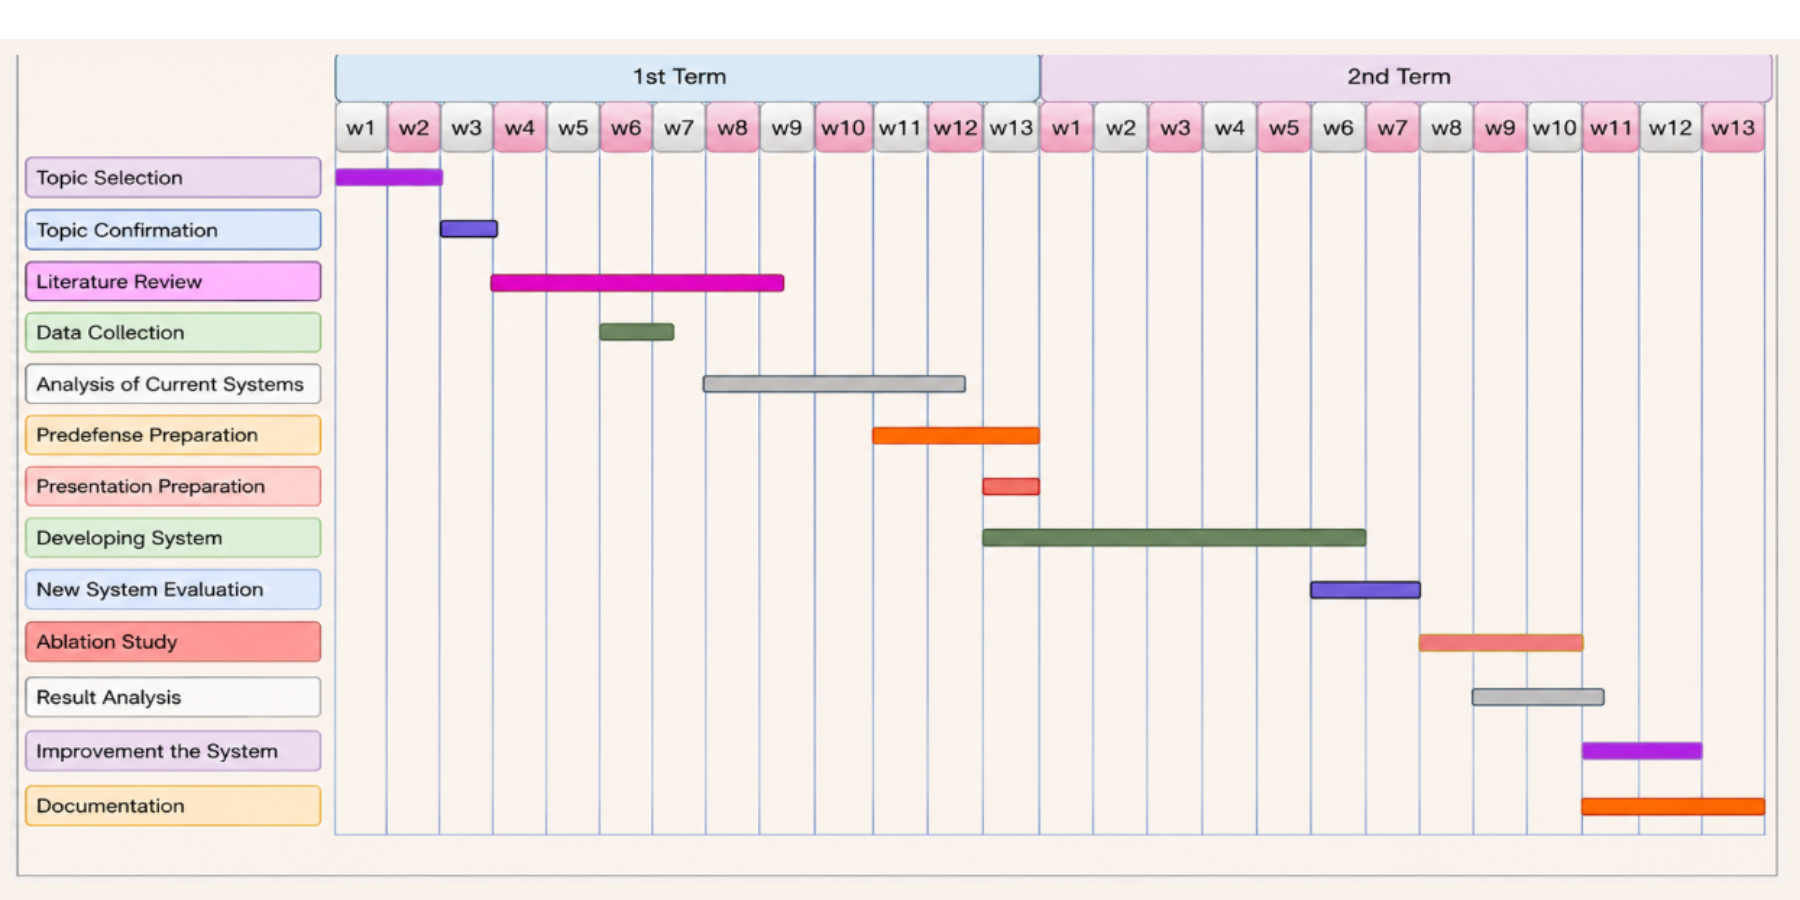
\includegraphics[width=1.0\textwidth]{img/workflow.png}
    \caption{Entire Project Workflow.}
    \label{fig:Entire Project Workflow}
\end{figure}

\subsection{Performance Analysis}

Performance testing looked at how responsive DASEMS is and how efficiently it moves through the evaluation workflow during a descriptive admission examination.

Because the architecture keeps the React frontend, Node.js backend, MongoDB database, and Python document processing service as separate pieces, the heavier work -- PDF processing and OCR -- runs on the Python service without dragging down the responsiveness of the web application itself.

The React frontend only re-renders what actually changes, and indexed MongoDB collections keep data retrieval fast. PDF processing and answer extraction both run asynchronously, so administrators and teachers can keep working while documents are being processed in the background.

The evaluation interface only pulls in answers that are actually assigned to a given teacher, which cuts down on unnecessary data loading, and the automated assignment and moderation modules let evaluation happen in parallel while keeping administrative overhead low.

\begin{table}[H]
\centering
\caption{Performance Analysis Summary}
\label{tab:performance_analysis}
\begin{tabular}{|p{6cm}|p{5cm}|p{2cm}|}
\hline
\textbf{Performance Aspect} & \textbf{Observation} & \textbf{Status} \\
\hline
Frontend Responsiveness & Smooth navigation and UI updates & Good \\
\hline
Backend API Response & Stable communication with frontend & Good \\
\hline
Database Operations & Fast retrieval using indexes & Good \\
\hline
PDF Processing & Executed asynchronously & Good \\
\hline
Teacher Assignment & Balanced workload distribution & Good \\
\hline
Evaluation Workflow & Parallel evaluation supported & Good \\
\hline
Moderation Process & Triggered only when required & Good \\
\hline
Overall System Integration & Stable during end-to-end workflow & Good \\
\hline
\end{tabular}
\end{table}
\FloatBarrier

Taken together, these observations suggest the system holds up well under the demands of a descriptive admission examination -- responsive and reliable throughout. The modular architecture, asynchronous PDF processing, efficient database design, and automated workflow all point toward a system that could scale to larger evaluations and eventually move to a cloud deployment.

\subsection{Discussion}

The results here show that DASEMS meets the objectives laid out back in Chapter I. Bringing together document processing, secure web technologies, and automated workflow management gives this system a real, practical answer to the problems universities run into when evaluating descriptive admission exams.

One of the bigger wins here is how much administrative work gets automated before evaluation even starts. The PDF processing module pulls question-wise answer images out of uploaded scripts on its own, so nobody has to manually separate questions, which saves a meaningful amount of prep time. The hybrid strategy -- pulling embedded PDF text where it exists, falling back to OCR where it doesn't -- keeps things efficient while still handling both searchable and scanned PDFs.

Keeping student identities hidden from teachers throughout evaluation makes the process fairer by design. On top of that, automated teacher assignment spreads answers out by subject specialization and workload, letting evaluation run in parallel while making sure no evaluator can see what the others scored.

Moderation adds another layer of reliability, but a targeted one -- only disputed evaluations actually reach the Head Examiner, so moderation doesn't become a bottleneck while consistency and transparency stay intact. The modular split between frontend, backend, document processing, and database also means the system is easier to maintain and has room to grow.

That said, the system isn't without its limits. The document processing module works from the assumption that exam layouts stay fairly consistent, so a script with a very different template would need extra configuration to handle. And to be clear, this system doesn't grade handwritten answers itself -- the actual academic judgment stays entirely with human examiners.

It's also worth noting that this prototype was tested in a controlled setting, using a representative but limited set of admission scripts. The results here point to the approach being workable, but rolling it out at full institutional scale would say a lot more about how it holds up over time and under heavier load.

Even with those caveats, DASEMS offers a clear step up from paper-based evaluation -- automated document processing, anonymous grading, centralized moderation, and automated results, all in one platform. And because of how it's built, there's a solid foundation here for adding things later, like AI-assisted handwriting recognition, smarter answer analysis, or a full cloud deployment.

\subsection{Chapter Summary}

This chapter covered the experimental evaluation of DASEMS -- functional testing, workflow validation, performance analysis, and a discussion of what it all means. Across the board, the evaluation confirmed that the system meets the objectives set out for this research.

Every major module -- authentication, PDF processing, question detection, answer extraction, teacher assignment, evaluation, moderation, and result generation -- worked correctly within the integrated system.

On the performance side, the modular architecture, asynchronous document processing, and optimized database operations kept the system responsive throughout the evaluation process, while automated teacher assignment and digital result generation added further gains in efficiency and transparency for descriptive admission examinations.

All told, DASEMS offers a practical, secure digital platform that cuts down manual administrative work considerably while making descriptive university admission examinations fairer and more efficient to run.

The next chapter closes out the thesis, summarizing the research contributions, discussing where the system falls short, and laying out directions for future work.
\include{Conclusions}


\newpage
\addcontentsline{toc}{section}{Reference}
\renewcommand\bibname{References}
\bibliographystyle{unsrt} 
\bibliography{References}
\nocite{*}


\end{document}